%%%%%%%%%%%%%%%%%%%%%%%%%%%%%%%%%%%%%%%%%%%%%%%%%%%%%%%%%%%%%%%%%%%%%%%%%%%%%%
%% Paying for Your Own Data:
%% A Closed-Loop Benchmark for Scientific ML Agents
%%
%% Target: Machine Learning: Science and Technology (IOP).
%% Compile with pdfLaTeX + BibTeX. See README.md.
%%
%% iopart.cls and its companions are redistributed here under the LPPL; they
%% are IOP Publishing's own class files, unmodified.
%%%%%%%%%%%%%%%%%%%%%%%%%%%%%%%%%%%%%%%%%%%%%%%%%%%%%%%%%%%%%%%%%%%%%%%%%%%%%%

\documentclass[12pt]{iopart}

\usepackage[T1]{fontenc}

% iopart.cls defines equation* itself (iopart.cls:788), which amsmath then
% tries to define again. Release the names before loading amsmath; amsmath's
% version is the one we want.
\makeatletter
\expandafter\let\csname equation*\endcsname\relax
\expandafter\let\csname endequation*\endcsname\relax
\makeatother
\usepackage{amsmath,amssymb}
\usepackage{booktabs}
\usepackage{array}
\usepackage{graphicx}
\usepackage{xcolor}
\usepackage{xspace}
\usepackage{enumitem}
\usepackage{url}
\usepackage[numbers,sort&compress]{natbib}
% iopart's thebibliography does not define \newblock, which the natbib
% bibliography styles emit between fields.
\providecommand{\newblock}{}
\usepackage{tikz}
\usetikzlibrary{positioning,arrows.meta,shapes.geometric,calc,fit,backgrounds}
\usepackage[colorlinks=true,linkcolor=black,citecolor=black,
            urlcolor=blue!55!black]{hyperref}
% Keep floats inside the section that discusses them. Without this, Figure 5
% drifted two pages earlier and appeared above the heading of the section it
% belongs to.
\usepackage[section]{placeins}

% MLST postdates this class file, so name it here.
\newcommand{\MLST}{{\it Mach. Learn.: Sci. Technol.}}

\setlist{nosep,leftmargin=1.4em}
%%%%%%%%%%%%%%%%%%%%%%%%%%%%%%%%%%%%%%%%%%%%%%%%%%%%%%%%%%%%%%%%%%%%%%%%%%%%%%
%% macros.tex -- notation, defined once and used consistently.
%%
%% The fill-in machinery of the conference draft is gone: every slot is closed.
%%%%%%%%%%%%%%%%%%%%%%%%%%%%%%%%%%%%%%%%%%%%%%%%%%%%%%%%%%%%%%%%%%%%%%%%%%%%%%

% --- physics -----------------------------------------------------------------
\newcommand{\psifield}{\psi}
\newcommand{\Rgrid}{R}
\newcommand{\Zgrid}{Z}
\newcommand{\Ip}{I_{\mathrm{p}}}
\newcommand{\rzero}{r_{0}}
\newcommand{\gs}{Grad--Shafranov}
\newcommand{\GS}{Grad--Shafranov}
\newcommand{\lcfs}{LCFS}

% --- the metric --------------------------------------------------------------
% Relative L2 appears on nearly every page; give it one spelling.
\newcommand{\relltwo}{\mbox{rel-$L_2$}}
\newcommand{\relLtwo}{\mbox{rel-$L_2$}}

% --- access levels and substrates --------------------------------------------
\newcommand{\Lzero}{\textsf{L0}}
\newcommand{\Lone}{\textsf{L1}}
\newcommand{\Ltwo}{\textsf{L2}}
\newcommand{\Lthree}{\textsf{L3}}
\newcommand{\hn}[1]{\textsf{#1}}

% --- code-ish ----------------------------------------------------------------
\newcommand{\code}[1]{\texttt{\small #1}}

\newcommand{\eg}{e.g.\xspace}
\newcommand{\ie}{i.e.\xspace}


\begin{document}

% \title[running head]{full title} -- iopart.cls:102
\title[Benchmarking coding agents on \GS{} surrogates]
      {Autokamak: Benchmarking coding agents on budgeted
       surrogate modelling of the \GS{} equation}

\author{Hindy Ros$^{1}$ and Deepjyoti Deka$^{2}$}
\address{$^{1}$ Massachusetts Institute of Technology, Cambridge, MA, USA}
\address{$^{2}$ MIT Energy Initiative, Massachusetts Institute of Technology,
         Cambridge, MA, USA}
\ead{hindyros@mit.edu}

\begin{abstract}
Benchmarks for coding and machine-learning agents almost always hand the agent
its data. We present a benchmark in which the agent must instead \emph{generate
its own data} from an expensive physics simulator under a fixed budget of
solver calls, and then ship a predictor that is scored independently on a
frozen set of cases it never sees. The task is surrogate modelling of the
\GS{} plasma equilibrium: the agent must learn to drive a finite-element
solver, design a sampling campaign, train a model mapping five plasma-shape
parameters to a $96\times64$ magnetic-flux field, and assess itself honestly.
Every condition emits the same machine-checkable deliverable, so any agent
substrate is scored on identical terms.

Across 59 runs on a single language model we find, first, that
\emph{giving an agent a proven library makes it worse}: from-scratch agents beat
library-assisted ones in all four substrates we tested (median \relltwo{}
$0.137$ against $0.229$; stratified rank test $z=-4.17$, permutation
$p\approx5\times10^{-5}$, blocked on substrate). A deterministic analysis of the
code each agent wrote explains why: given a library, all four substrates settle
on its default model and its named acquisition strategies; given nothing, all
four converge on a different method family, and two of them beat the library's
own score.

Our central finding concerns verification. \textbf{Fifteen of 49 scored runs
passed every contract gate while being physically invalid} --- a rate that
depends strongly on the agent substrate and not at all on how much scaffolding
it was given. The failures are not subtle once looked for: one run scored
$0.071$, better than most of the corpus, while emitting a magnetic field
throughout the vacuum region where the field is undefined. Self-reported error
diverges from independently measured error by up to $0.93$, and the runs that
misreport are largely \emph{not} the runs that are invalid, so neither
measurement detects the other. Machine-checkable deliverable contracts, the
standard instrument in this literature, detect none of it. We therefore
separate three questions a benchmark must ask --- did the agent deliver, is the
artifact physically valid, and did it tell the truth --- and measure all three,
alongside a fourth: did it build what it said it built.
\end{abstract}

\noindent{\it Keywords}: agent benchmarks, large language models, surrogate
modelling, active learning, plasma equilibrium, scientific machine learning

\submitto{\MLST}
\maketitle

\section{Introduction}
\label{sec:intro}

Benchmarks for machine-learning agents have settled into a shape. You give the
agent a dataset and a metric, and you see how good a model it can fit. MLE-bench
draws its tasks from Kaggle competitions; MLAgentBench, DSBench,
ScienceAgentBench and their relatives vary the domain and the scaffolding but
keep the shape.\footnote{Citations are collected in
Section~\ref{sec:related}.} In every case the data exists before the agent
starts, and it is the same data for every agent. That is exactly what makes
those benchmarks clean comparisons.

It is also what makes them unlike most of computational science. There, the
expensive step is usually \emph{getting} the data --- running the simulation,
performing the experiment, doing the solve --- and the decision that separates a
good researcher from a mediocre one is \emph{where to spend the next unit of
budget}. An agent that is excellent at fitting a dataset it was handed may be
useless at deciding which experiments are worth running. Nothing in the current
crop of benchmarks would tell us either way.

This paper introduces a benchmark that puts that decision back. The agent is
given a physics solver, a five-dimensional space of inputs, and a hard budget of
solver calls. It must work out how to drive the solver, decide which points in
the space to spend its budget on, train a model on what it collected, and hand
over a predictor --- which we then score, on a set of cases it has never seen,
with machinery it does not control (Figure~\ref{fig:loop}).

\begin{figure}[t]
\centering
\resizebox{\textwidth}{!}{%
\begin{tikzpicture}[
  font=\small,
  box/.style={draw=black!55, rounded corners=2pt, align=center, inner sep=4pt,
              minimum height=9mm, text width=30mm},
  ag/.style={box, fill=blue!6,   draw=blue!60},
  sv/.style={box, fill=orange!8, draw=orange!70},
  ev/.style={box, fill=green!8,  draw=green!45!black},
  dl/.style={box, fill=black!4},
  fl/.style={-{Stealth[length=2mm]}, draw=black!70, thick},
  lb/.style={font=\scriptsize\itshape, text=black!60},
  hd/.style={font=\scriptsize\bfseries, text=black!70},
]

% ---- left: inside the evaluated cell ----
\node[dl] (task)  at (0,0)      {frozen task spec\\[1pt]{\scriptsize 5 parameters $\cdot$ solve budget\\ process gates}};
\node[ag] (agent) at (0,-2.1)   {agent harness\\[1pt]{\scriptsize \Ltwo{} library-assisted\\ \Lthree{} from scratch}};
\node[sv] (solv)  at (5.4,-2.1) {TokaMaker\\[1pt]{\scriptsize \GS{} FE solver}};
\node[dl] (deliv) at (0,-4.6)   {deliverable\\[1pt]{\scriptsize \code{report.json}\\ \code{predict.py}}};

\draw[fl] (task) -- (agent);
\draw[fl] ([yshift=3.5mm]agent.east) -- ([yshift=3.5mm]solv.west)
      node[midway,above,lb]{params};
\draw[fl] ([yshift=-3.5mm]solv.west) -- ([yshift=-3.5mm]agent.east)
      node[midway,below,lb]{$\psi$ or failure};
\draw[fl] (agent) -- (deliv);

\node[lb, text width=36mm, align=center] at (5.4,-3.2)
     {$\le 450$ solves, 3 adaptive rounds};

% ---- separator ----
\draw[dashed, black!45] (7.7,1.0) -- (7.7,-5.5);
\node[hd, anchor=south] at (2.7,0.85) {inside the evaluated cell};
\node[hd, anchor=south] at (10.9,0.85) {independent evaluation};

% ---- right: evaluation the agent never sees ----
\node[ev] (gates) at (10.9,-0.4) {contract gates\\[1pt]{\scriptsize did it deliver?}};
\node[ev] (score) at (10.9,-2.5) {frozen test set\\[1pt]{\scriptsize 60 held-out solves\\ relative $L_2$}};
\node[ev] (diag)  at (10.9,-4.6) {diagnostics\\[1pt]{\scriptsize valid? honest?}};

\coordinate (bus) at (8.6,-4.6);
\draw[fl] (deliv.east) -- (bus);
\draw[fl] (bus) -- (diag.west);
\draw[fl] (bus) |- (score.west);
\draw[fl] (bus) |- (gates.west);

\end{tikzpicture}%
}
\caption{The benchmark loop. Everything inside the dashed line is the agent's
own business: it is handed a frozen task specification and a solver, and it must
decide which equilibria to compute, spending a fixed budget across an initial
design and up to three adaptive rounds. What it hands over is a small set of
files. Everything to the right of the dashed line happens outside the agent's
reach --- the files are checked mechanically, the predictor is run on sixty
held-out cases the agent never sees, and the result is put through diagnostics
that ask whether the field is physically meaningful and whether the agent's own
report of its performance was true. Every condition in this paper, including
the two that use no language model at all, passes through that identical
right-hand column.}
\label{fig:loop}
\end{figure}

\paragraph{Why this particular solver.}
The ground truth comes from TokaMaker~\citep{hansen2024tokamaker}, a
finite-element solver for the equilibrium of a magnetically confined fusion
plasma. Section~\ref{sec:physics} explains the physics from scratch; the
properties that make it a good instrument for measuring agents are these. It is
\emph{genuinely expensive} --- seconds per solve, so a budget bites. It
\emph{fails}, and does so as a function of the inputs, so the feasible region
has to be discovered rather than assumed. Its output is
\emph{high-dimensional} (a field on a $96\times64$ grid) while its input is
five numbers, so dimensionality reduction is a real design decision rather than
a formality. It is \emph{unforgiving about physics}: the quantity being
predicted is a signed physical field in webers, undefined outside the plasma, so
an agent that quietly normalises it, or fills in the region where it does not
exist, produces something that looks plausible and is wrong. And the answers are
\emph{not memorisable} --- these particular equilibria are not on the internet.

\paragraph{What we found.}
Three things, in increasing order of how much they surprised us.

First, with the language model held fixed across every condition, \emph{which
agent framework you use matters more than how much help you give it}. The
per-cell medians span a factor of $8.8$ across four substrates, against a factor
of $1.7$ between the two levels of scaffolding.

Second, \emph{the scaffolding helped in the wrong direction}. Agents allowed to
import a proven, tested pipeline library did worse than agents made to write
everything themselves --- in all four substrates, with no exceptions. A
deterministic analysis of the code they wrote (Section~\ref{sec:agentlogic})
says why, and it is not that the library is bad: given the library, all four
substrates adopt its default model and the acquisition strategies its
documentation names; given nothing, all four independently find a different
method family, and two of them beat the library's own score on the same test
set.

Third, and this is the finding we think matters beyond this benchmark:
\textbf{31\% of the runs that passed every machine-checkable gate were
physically invalid}. Not marginal --- invalid. One of them scored better than
most of the corpus on the error metric while emitting a magnetic field
throughout the vacuum region outside the plasma, where the field is not defined
at all (Figure~\ref{fig:pva}, second row). The contract that certified it is the
standard instrument in this literature: check the files exist, check they parse,
check the predictor runs and returns the right shape. It cannot see this class
of failure, and neither can the headline error number.

\paragraph{Contributions.}
\begin{enumerate}
\item \textbf{A closed-loop scientific-ML benchmark} in which the agent buys its
  own training data from an expensive solver under a fixed budget, with a
  machine-checkable deliverable, independent scoring on a frozen set, and a
  four-rung ladder of scaffolding from a zero-LLM scripted policy to
  from-scratch --- every rung inside the identical contract
  (Section~\ref{sec:benchmark}).
\item \textbf{A model-controlled comparison of four agent frameworks.} Every
  cell runs the same model, so ``which framework'' is not confounded with
  ``which model'' --- a confound we had in our own earlier campaigns
  (Section~\ref{sec:results}).
\item \textbf{A verification layer} that separates delivery, physical validity
  and self-report honesty, and finds all three come apart
  (Section~\ref{sec:verification}).
\item \textbf{A deterministic, LLM-free account of what each agent actually
  built} --- its chain of methods, its per-round decision logic, and whether its
  code agrees with its own prose. This is what makes the scaffolding result
  interpretable rather than merely surprising (Section~\ref{sec:agentlogic}).
\end{enumerate}

\section{The problem, for a reader who has never seen a tokamak}
\label{sec:physics}

This section explains the physics the benchmark is built on. A plasma physicist
can skip it; nothing later depends on more than is written here.

\subsection{What is being computed, and why anyone wants it fast}

A tokamak confines a hot plasma inside a doughnut-shaped magnetic field. For
the plasma to sit still rather than drift into the wall, the outward pressure of
the gas has to be balanced everywhere by the inward force of the magnetic field.
A configuration in which that balance holds is called an \emph{equilibrium}, and
finding it is the first thing anyone does when designing a device, planning a
discharge, or controlling one in real time.

Because a tokamak is (to a very good approximation) symmetric about its central
axis, the three-dimensional problem collapses to two dimensions: a single
cross-sectional slice, with coordinates $\Rgrid$ measured outward from the axis
of symmetry and $\Zgrid$ measured vertically. On that slice the force balance
becomes one elliptic partial differential equation, the \GS{}
equation~\citep{grad1958hydromagnetic,shafranov1958magnetohydrodynamical}:
\begin{equation}
  \Delta^{*}\psi \;=\; -\mu_{0}R^{2}p'(\psi) \;-\; F(\psi)F'(\psi),
  \qquad
  \Delta^{*} \;\equiv\;
  \frac{\partial^{2}}{\partial R^{2}}
  - \frac{1}{R}\frac{\partial}{\partial R}
  + \frac{\partial^{2}}{\partial Z^{2}} .
  \label{eq:gs}
\end{equation}

The unknown $\psi(R,Z)$ is the \emph{poloidal flux function}, measured in
webers. Two facts about it are all that the rest of this paper needs.

\textbf{The contours of $\psi$ are the surfaces the plasma lives on.} Magnetic
field lines lie within surfaces of constant $\psi$, so a plot of $\psi$ is a
picture of the magnetic structure: a set of nested closed loops around a central
peak. Figure~\ref{fig:primer}(b) is a real solution. The outermost closed
contour is the plasma boundary, conventionally the \emph{last closed flux
surface} or \lcfs{}.

\textbf{Outside that boundary, $\psi$ is not defined here.} We solve the
\emph{fixed-boundary} problem: the boundary shape is prescribed, and the
equation is solved on the region inside it. There simply is no value at grid
points outside, and the solver returns \texttt{NaN} there. About 80\% of the
grid is \texttt{NaN} in a typical case. This sounds like a bookkeeping detail.
It is the single most consequential convention in the benchmark, and
Section~\ref{sec:verification} is largely about what agents do with it.

\paragraph{Why a surrogate model is worth having.}
A finite-element \GS{} solve takes seconds. That is fine once, and ruinous
inside a loop. Device design searches over shapes; scenario planning sweeps over
operating points; real-time shape control needs an equilibrium every
millisecond, and the iterative solve is precisely the latency bottleneck that
prevents higher-bandwidth control. Learning a fast approximation of the
solver --- a \emph{surrogate} --- is therefore an active line of work in its own
right, with recent efforts targeting millisecond-scale neural-operator
equilibria~\citep{krastev2026millisecond} and control-oriented surrogates
validated on an operating device~\citep{grandin2026experimental}. The task we
set the agents is a scaled-down version of a problem people are actually paid to
solve.

\subsection{The five numbers that define a case}

The boundary is a D-shape, the standard cross-section of a modern tokamak,
described by four geometric parameters plus the current flowing in the plasma
(Figure~\ref{fig:primer}(a)):

\begin{center}
\footnotesize
\begin{tabular}{@{}llll@{}}
\toprule
\textbf{Symbol} & \textbf{Name} & \textbf{Range} & \textbf{What it does} \\
\midrule
$\rzero$  & major radius   & $0.35$--$0.55$\,m & how far the doughnut's centre sits from the axis \\
$a$       & minor radius   & $0.10$--$0.20$\,m & how fat the doughnut is \\
$\kappa$  & elongation     & $1.0$--$1.6$      & vertical stretch; $1$ is a circle \\
$\delta$  & triangularity  & $0.0$--$0.4$      & pulls the top and bottom inward into a D \\
$\Ip$     & plasma current & $80$--$200$\,kA   & sets the overall magnitude of $\psi$ \\
\bottomrule
\end{tabular}
\end{center}

\noindent Figure~\ref{fig:primer}(c) shows what the two shape parameters do.
The task, then, is to learn the map
\begin{equation}
  (\rzero, a, \kappa, \delta, \Ip) \;\longmapsto\; \psi(R,Z)
  \in \mathbb{R}^{96\times64},
\end{equation}
from a budget of solver calls the agent itself chooses.

\begin{figure}[t]
\centering
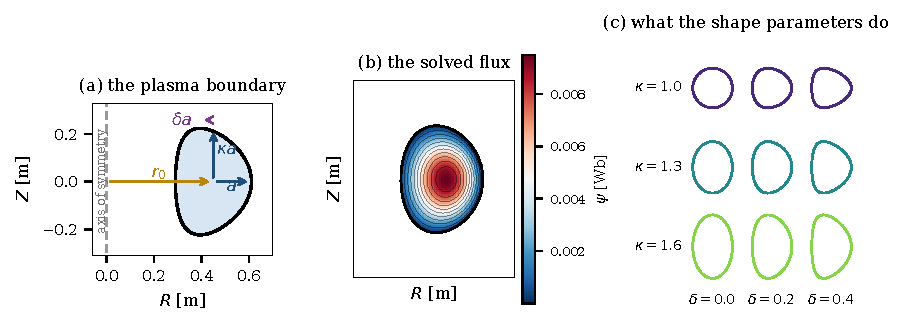
\includegraphics[width=\textwidth]{figures/fig_primer}
\caption{\textbf{(a)} The plasma boundary and the four shape parameters that set
it; the fifth, the plasma current $\Ip$, scales the field rather than the shape.
\textbf{(b)} A real solution from the frozen test set. Colour is the poloidal
flux $\psi$; the black contours are flux surfaces, and the heavy line is the
plasma boundary. Outside it, $\psi$ is undefined and the solver returns
\texttt{NaN} --- roughly 80\% of the grid. \textbf{(c)} What elongation and
triangularity do to the boundary: $\kappa$ stretches it vertically, $\delta$
pulls the top and bottom inward.}
\label{fig:primer}
\end{figure}

\subsection{How good is a prediction? Reading the error metric}

Predictions are scored by relative $L_2$ error, computed per case over the grid
points where the truth is defined:
\begin{equation}
  \relltwo_i \;=\;
  \frac{\bigl\lVert \hat{\psi}_i - \psi_i \bigr\rVert_2}
       {\bigl\lVert \psi_i \bigr\rVert_2},
  \qquad
  \text{over } \{(\Rgrid,\Zgrid) : \psi_i(\Rgrid,\Zgrid) \text{ finite}\}.
  \label{eq:rell2}
\end{equation}
Zero is perfect. The number that gives it meaning is what you get for free: a
predictor that ignores its input entirely and always returns the average flux
map of the training set scores $0.4933$ on our test set. We call that the
\emph{mean-map baseline} and quote accuracy against it,
$100\times(1 - \relltwo/0.4933)$, so that $0\%$ means ``no better than not
trying'' and $100\%$ means exact.

Because an error metric is easier to trust once you have seen it,
Figure~\ref{fig:errorcal} shows the same equilibrium predicted at a range of
\relltwo{} values by actual runs from our campaign. Below about $0.1$ the
prediction is visually indistinguishable from the truth. By $0.2$ the field is
noticeably blurred. At the mean-map baseline it is a smear with no case-specific
structure at all, and beyond that the predictor is contributing nothing.

\begin{figure}[t]
\centering
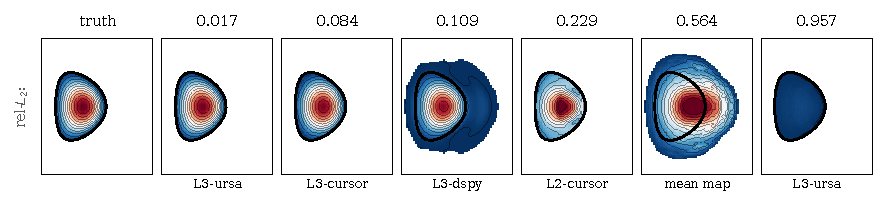
\includegraphics[width=\textwidth]{figures/fig_error_calibration}
\caption{What the error metric looks like. The same test equilibrium, predicted
by six actual runs spanning the range we observed, with \relltwo{} for that case
above each panel and the condition that produced it below. ``Mean map'' is the
input-independent baseline. All panels share a colour scale.}
\label{fig:errorcal}
\end{figure}

\section{Related work}
\label{sec:related}

\paragraph{Benchmarks that hand the agent its data.}
The dominant shape gives an agent a repository or a dataset and scores the
artifact it produces. SWE-bench~\citep{jimenez2024swebench} scores patches
against held-out tests; AgentBench~\citep{liu2024agentbench} covers interactive
environments more broadly. Closest to our setting are the ML-engineering
suites: MLE-bench~\citep{chan2024mlebench} runs agents on Kaggle competitions
and grades against the private leaderboard;
MLAgentBench~\citep{huang2024mlagentbench} scores iterative experimentation on
fixed task datasets; DSBench~\citep{jing2024dsbench} draws on data-science
competitions.

A second line targets science specifically.
ScienceAgentBench~\citep{chen2025scienceagentbench} assembles data-driven
discovery tasks from published papers;
DiscoveryBench~\citep{majumder2025discoverybench} formalises hypothesis search
over provided datasets; BixBench~\citep{mitchener2025bixbench} does the same for
computational biology; CORE-Bench~\citep{siegel2024corebench} scores
computational reproducibility; PaperBench~\citep{starace2025paperbench} scores
replication of ML papers; RE-Bench~\citep{wijk2024rebench} pits agents against
human experts on open-ended research engineering.

These differ enormously in domain and open-endedness, and in one respect they
agree: the training data exists in advance and is identical for every agent.
That is what makes them clean comparisons --- and it is also what removes
acquisition from the set of decisions being measured.

\paragraph{The literature the task asks an agent to rediscover.}
Deciding where to measure next is of course a mature field. Active
learning~\citep{settles2009active} and Bayesian experimental
design~\citep{chaloner1995bayesian} supply the strategies a competent agent
might reach for --- uncertainty sampling, residual-targeted acquisition,
variance reduction under a probabilistic model --- and space-filling designs
such as Latin hypercubes~\citep{mckay1979lhs} supply the baseline those
strategies have to beat. We contribute nothing to that literature. What we
measure is whether an agent reaches for any of it unprompted, implements what it
says it implemented, and spends a hard budget sensibly
(Section~\ref{sec:agentlogic}).

\paragraph{What we add, stated narrowly.}
The gap is not that nobody acquires data. It is that \emph{agentic coding
benchmarks do not make the acquisition policy part of what is scored}. To our
knowledge, as of mid-2026, no existing agent benchmark requires the agent to
(i) drive an expensive, failure-prone numerical solver for which it has not been
handed a working harness, (ii) allocate a hard budget across adaptive rounds,
and (iii) be scored on a frozen set it never sees, with a zero-LLM scripted
policy running inside the identical contract as the reference point.

Two recent works come closest. AstaBench~\citep{bragg2025astabench} assembles a
large scientific-agent suite and is motivated by the same complaint about
confounders --- model cost and tool access varying across compared systems ---
that motivates our model control; it supplies the tools and the data rather than
scoring acquisition. And a position paper argues that the execution harness,
not the model it wraps, is often the binding constraint on agent
performance~\citep{zhang2026harness}. Our campaign is a direct empirical test of
that claim: one model, four harnesses, and the spread measured
(Section~\ref{sec:harness-effect}).

\paragraph{The agent frameworks we evaluate.}
These are existing systems, not contributions of this paper:
URSA~\citep{ursa2025}, a planner/executor pair built on LangGraph, part of the
LangChain project~\citep{langchain2022}; DSPy~\citep{khattab2024dspy}, whose
typed modules we also use for the \Lone{} decision layer and whose GEPA
optimiser~\citep{agrawal2025gepa} we use for prompt optimisation; and two
commercial command-line coding agents. We evaluated them as we found them; none
of their authors was involved in or consulted about this evaluation.

\section{The benchmark}
\label{sec:benchmark}

\subsection{Vocabulary}
\label{sec:notation}

Five terms recur, and it is worth fixing them before they are used.

\begin{center}
\footnotesize
\begin{tabular}{@{}lp{0.66\textwidth}@{}}
\toprule
\textbf{Term} & \textbf{Meaning in this paper} \\
\midrule
\emph{harness} (or \emph{substrate})
  & The agent framework: the software that wraps a language model and turns it
    into something that can read files, run commands and iterate. We compare
    four. It is not the model. \\
\emph{access level}
  & How much pre-written help the agent is given, from \Lzero{} (a scripted
    policy, no model at all) to \Lthree{} (write everything yourself).
    Section~\ref{sec:ladder}. \\
\emph{the contract}
  & The fixed set of machine-checkable conditions every condition's output must
    satisfy: the files exist, the report parses, the predictor runs and returns
    the right shape on the right grid. Section~\ref{sec:contract}. \\
\emph{the frozen set}
  & Sixty solved equilibria, fixed once and never regenerated, on which every
    predictor in this paper is scored. No agent ever sees them. \\
\emph{honesty gap}
  & An agent's own reported error minus its independently measured error.
    Negative means it claimed to be better than it was.
    Section~\ref{sec:honesty}. \\
\bottomrule
\end{tabular}
\end{center}

\subsection{What the agent is asked to do}
\label{sec:task}

Each agent receives a frozen, versioned problem statement --- the same text for
every replicate, hashed into every run record, and reproduced verbatim in
Appendix~\ref{app:tasktext}. It specifies five things.

\textbf{The forward problem.} Fixed-boundary equilibria of D-shaped plasmas in
the five parameters of Section~\ref{sec:physics}, over the stated ranges, at the
solver's default profile shapes.

\textbf{A campaign structure with a hard budget.} At most 150 solves for an
initial space-filling design, then up to three adaptive rounds of exactly 100
new solves each. Failed solves count against the budget. Crucially, each round's
points must be chosen from the current model or the data collected so far: a
single large one-shot design is explicitly ruled out, because the object of
study is the choice of where to sample.

\textbf{A stopping criterion.} Keep a validation set separate from the test set,
and stop early once validation error falls to $0.30\times$ the mean-predictor
baseline or better.

\textbf{An honest evaluation requirement.} Hold out at least 20 solves at random
parameters with a recorded seed, and never use them for training, model
selection or acquisition.

\textbf{A self-assessment requirement.} Report whether the adaptive sampling
actually helped, ``or an honest statement that it did not''.

Four process gates are mandatory and identical for every condition: a
\emph{meshing milestone} (reproduce the solver's own worked example before
generalising), a \emph{pilot gate} (at least 20 solves at 50\% success before
the rounds begin), a \emph{storage-validation gate} (a solve counts as
successful only once its stored file has been read back and confirmed to contain
finite numbers), and a \emph{deliverable self-test} (run every documented
command in a fresh process before declaring done). The last two were added after
an earlier campaign in which an agent stored all-\texttt{NaN} data, counted it as
success, and shipped a predictor it had never executed.

\subsection{The deliverable contract}
\label{sec:contract}

Every condition emits the same three files --- \code{report.json},
\code{predict.py}, \code{README.md} --- and they are checked mechanically
(Table~\ref{tab:gates}). \code{contract.passed} is the flat \textsc{and} of
every gate: no weighting, no partial credit.

\begin{table}[t]
\caption{The deliverable contract. The scoring subprocess is stripped of
provider credentials, so \code{predict.py} must work offline, and it runs in its
own process group so a timeout reaps the solver's children too. The final gate
applies only at \Lthree{}, so \Lthree{} runs face nine checks and \Ltwo{}
eight.}
\label{tab:gates}
\footnotesize
\begin{tabular}{@{}ll@{}}
\toprule
\textbf{Gate} & \textbf{What it checks} \\
\midrule
\code{artifact:report.json} & present and non-empty \\
\code{artifact:predict.py}  & present and non-empty \\
\code{artifact:README.md}   & present and non-empty \\
\code{report\_parses}       & \code{report.json} is valid JSON \\
\code{report\_keys}         & the required keys are \emph{present} \\
\code{predict\_runs}        & \code{python predict.py -{}-input p.json -{}-output o.npz} exits 0 \\
\code{predict\_shape}       & the returned \code{psi} is $(N, 96, 64)$ \\
\code{predict\_grid}        & the returned \code{R}, \code{Z} match the frozen axes to $10^{-9}$ \\
\code{no\_autotokamak\_import} & \Lthree{} only: no workspace file imports the platform library \\
\bottomrule
\end{tabular}
\end{table}

One design choice in that table does a great deal of work later.
\code{report\_keys} \textbf{checks that the agent's self-reported metrics are
present, and never that they are correct}. The agent's own numbers are recorded
verbatim and never cross-checked by the contract. That is what makes the
honesty measurement of Section~\ref{sec:honesty} possible at all: we can compare
what the agent said about itself against what we measured, precisely because
nothing in the pipeline ever forced the two to agree.

Predictions are scored on the frozen set of 60 parameter vectors described in
Section~\ref{sec:physics}, using Equation~\eqref{eq:rell2}. One detail matters:
\textbf{a \texttt{NaN} prediction at a point where the truth is defined is
scored as a full-magnitude miss}, never skipped. Skipping would let an
all-\texttt{NaN} prediction score as perfect.

\subsection{The scaffolding ladder}
\label{sec:ladder}

The benchmark's second axis is how much help the agent gets. All four rungs emit
the identical contract and are scored on the identical frozen set, which is what
makes them comparable at all.

\begin{center}
\footnotesize
\begin{tabular}{@{}llp{0.52\textwidth}@{}}
\toprule
\textbf{Level} & \textbf{Name} & \textbf{What the agent does} \\
\midrule
\Lzero{}  & scripted         & Nothing. A seeded heuristic policy drives a pre-written pipeline; no language model is involved at any point. \\
\Lone{}   & structured       & A model makes only typed decisions --- which model family, how many components, what to do next --- inside fixed pipeline code. \\
\Ltwo{}   & library-assisted & The agent writes the glue code and \emph{may} import the platform library, which already implements the sweep, the acquisition strategies and the model zoo. \\
\Lthree{} & from-scratch     & The agent writes everything. Importing the platform library is forbidden, and the prohibition is audited by static analysis of every file it wrote. \\
\bottomrule
\end{tabular}
\end{center}

\Lzero{} is the reference point that makes the rest interpretable. It is
deterministic, it costs nothing, and it is scored by the same scorer on the same
cases. Without a zero-model condition inside the same contract there is no way
to say how much of a given score is the task being easy and how much is the
agent being good.

\subsection{Is the task hard for the right reasons?}
\label{sec:characterisation}

Before asking whether agents can do this, it is worth establishing that the
task rewards the thing we claim it rewards. Three facts, established by a
direct sweep of 9993 converged solves independent of any agent, are shown in
Figure~\ref{fig:taskchar}; the underlying tables are in
Appendix~\ref{app:characterisation}.

First, error falls with training-set size and saturates --- and \emph{the best
model family changes along the way}, from polynomial ridge up to $N=200$ to
kernel ridge from $N=400$ on. Model selection is therefore a real decision that
depends on the data the agent chose to collect, not a fixed answer that can be
looked up. The agents' 450-solve budget sits in the part of that curve where it
still matters.

Second, at a matched budget, \emph{where} you sample beats \emph{how much}.
Space-filling designs beat uniform random by 21\% at $N=100$, narrowing to 6\%
by $N=1600$; deliberately clustered sampling is catastrophic at every budget.
Coverage is the first-order concern and its value decays as the budget grows.

Third, and this is what makes the sampling decision consequential rather than
cosmetic: \emph{outside its training region the surrogate collapses}. Train on
half the parameter space and test on the other half and the error ratio is
$0.94$ --- no better than predicting the mean field --- against $0.38$--$0.40$
within distribution. An agent that samples badly does not lose a few percent.
It produces a model that fails completely off-distribution and, because it
evaluates itself on its own test set drawn from its own sampling distribution,
it may never find out.

\begin{figure}[t]
\centering
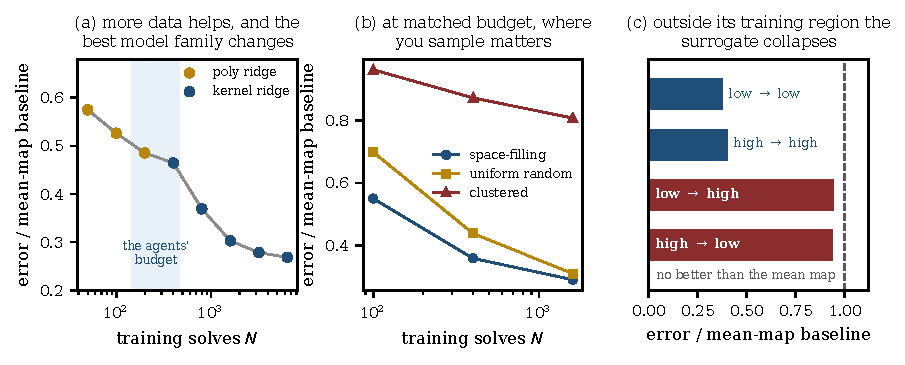
\includegraphics[width=\textwidth]{figures/fig_task_character}
\caption{The task is hard for the right reasons. \textbf{(a)} Error against
training-set size, with the best model family at each size marked; the shaded
band is the agents' campaign budget. \textbf{(b)} At matched budget, sampling
strategy dominates. \textbf{(c)} Trained on one half of the parameter space and
tested on the other, the surrogate is no better than the mean map. All values
are relative $L_2$ divided by the mean-map baseline, from a pool of 9993
converged solves.}
\label{fig:taskchar}
\end{figure}

\subsection{A worked example}
\label{sec:worked}

To make the loop concrete, here is one run end to end:
\Lthree{}-\hn{cursor} replicate~2, chosen because it is unremarkable --- it sits
in the middle of its cell and nothing went wrong.

It received the task text of Section~\ref{sec:task} and a workspace containing
nothing but a read-only copy of the solver's source tree. It began, as
instructed, by locating the solver's own fixed-boundary example and reproducing
it as a standalone script (\code{meshing\_milestone.py} in its workspace),
confirming it could produce a finite flux field before writing anything of its
own. It then built a mesh-and-solve wrapper, ran a 20-solve random pilot to
check the failure rate against the mandated 50\% threshold, and extended to 150
attempted solves with a Latin hypercube over the five parameters. It set aside
a further 30 solves for validation and 25 for its own held-out test, and
recorded a separate seed for each of the four.

For the model it chose something no prompt suggested: a PyTorch multilayer
perceptron mapping the five parameters directly to the $96\times64$ field,
trained under a loss masked to the points inside the plasma. It left dropout
active at inference so that repeated forward passes give a spread, and used
that spread as its acquisition signal --- sampling where the dropout ensemble
disagreed most. One adaptive round of 100 solves was enough: validation error
crossed the task's $0.30\times$-baseline threshold and it stopped early, having
used 305 of its 450 permitted solves.

It wrote the three required files, re-ran its own \code{predict.py} in a fresh
process as instructed, and declared itself done after 8.9 minutes and about
\$1.64 of model spend. Our independent scoring found \relltwo{} $0.0622$ ---
87.4\% accuracy against the mean-map baseline, the fourth-best run in the
campaign. All nine gates passed, all four physical-validity diagnostics passed,
and its \texttt{NaN} mask agreed with ground truth on 99.98\% of grid points.
Its own report claimed $0.0611$ against our $0.0622$: a gap of $-0.001$, which
is to say it flattered itself by a tenth of a percent. It also volunteered,
unprompted, that its adaptive round had helped --- $0.085$ before, $0.061$
after.

That is what the benchmark looks like when everything works. Much of the rest of
this paper is about the runs where it did not, and about how little the contract
noticed.

\section{Experimental design}
\label{sec:design}

\subsection{Conditions}

The campaign is the cross of two access levels and four agent frameworks:
$\{\Ltwo{}, \Lthree{}\} \times \{\hn{ursa}, \hn{dspy}, \hn{pi}, \hn{cursor}\}$,
eight cells, replicated --- plus a budget-matched \Lzero{} reference arm. We
attempted 59 runs and scored 49.

Replicate counts are deliberately unequal: two substrates at $n=10$ and two at
$n=5$. The campaign was budgeted in dollars rather than in runs, and one
substrate costs an order of magnitude more per run than another
(Section~\ref{sec:cost}). Failures reduce some cells further. Every denominator
in this paper counts \emph{attempts}, not survivors, which is the conservative
choice and is stated wherever a rate appears.

\subsection{Holding the model fixed}

Every cell runs the same language model, \code{gpt-5.2}. This is the point of
the design. In an earlier campaign of our own, one harness ran a different
model family from the others, and the resulting comparison was uninterpretable:
any difference could have been the framework or the model, and nothing in the
data could separate them.

Pinning it is fiddlier than it sounds, because the four adapters disagree about
how a model is named --- two take \code{openai:gpt-5.2}, one takes
\code{openai/gpt-5.2}, and the command-line agent takes a bare \code{gpt-5.2}.
We pin the name per adapter inside the frozen task specification rather than
passing a single command-line override, so that the model string is recorded
three independent times per run and the control is auditable after the fact. A
fifth adapter we maintain is excluded from the campaign entirely for the same
reason: it cannot run the pinned model, and including it would have reintroduced
exactly the confound the design exists to remove.

Framework versions were \hn{ursa} 0.15.1, \hn{dspy} 3.2.1, \hn{pi} 0.73.1 and
\hn{cursor} 2026.09.18, against Open FUSION Toolkit 26.6. Those are recorded
from the machine, not from the run records --- which stamp the task hash, the
prompt version, the model and the replicate index, but not the substrate's own
version. That is a gap in our harness and we would close it in a future
campaign.

\subsection{Equal compute budgets, and why they are hard to enforce}
\label{sec:budgets}

Giving every substrate the same budget turned out to be the hardest engineering
requirement in the benchmark, and the failure modes generalise well past this
paper.

Two adapters accepted a \code{timeout\_seconds} argument and silently ignored
it. Fixing that exposed two deeper problems. First, \textbf{a timeout raised as
an ordinary exception is swallowed}: agent frameworks wrap their step loops in
broad \code{except Exception} handlers and treat anything caught as a
recoverable step failure, so a timeout delivered by signal vanishes into the
agent's own retry logic --- and because \code{signal.alarm} is one-shot, a
single swallowed alarm disables the cap permanently. One harness absorbed its
90-minute cap this way and ran for over ten hours. Second, \textbf{killing the
agent process does not stop the work}: Python's \code{subprocess.run}, called
with a timeout, kills the direct child and then waits on its pipes again --- but
the solver's grandchildren inherit those pipes and hold them open, so the
timeout path itself blocks. One cell sat in that deadlock for 9 hours 19
minutes.

The fixes are to raise a \code{BaseException} subclass, for the same reason
\code{KeyboardInterrupt} is one, and to run each agent in its own process group
and signal the group. The general lesson is worth stating plainly: \textbf{an
agent harness is third-party code and cannot be trusted to honour a deadline
from inside}. We enforce the budget at three independent levels --- in-adapter,
by process-group kill, and by a driver-side watchdog that nothing running inside
the cell can intercept.

We also equalised the outer feedback-round setting to 1. Only two of the four
adapters implement outer review-and-fix rounds at all, so any higher value hands
those two a second pass the others never get --- an arbitrary two-tier design
that was the mechanical cause of their longer runtimes and larger spend in
earlier campaigns. One is the only value all four honour identically.

\subsection{What is held fixed}

The prompt text (version 3, hashed per run), the evaluation grid, the
60-parameter test set, the gate set and the scoring rule. The \Ltwo{} and
\Lthree{} problem statements are byte-identical except for ten passages, every
one of which concerns access level; they are reproduced with the differences
marked in Appendix~\ref{app:tasktext}. Results are pooled only within one prompt
version and one scoring epoch, and the aggregation tool refuses to mix them.

\subsection{Analysis, and one change we made after seeing the data}
\label{sec:analysis}

The unit of analysis is the cell. Pass rates carry Wilson score
intervals~\citep{wilson1927probable}, which --- unlike the normal
approximation --- do not collapse to zero width at $0/n$ or $n/n$.
Relative-$L_2$ is summarised by medians with percentile bootstrap
intervals~\citep{efron1979bootstrap} rather than means, because a single
catastrophic replicate makes a mean uninterpretable and we have several.

The \Ltwo{}/\Lthree{} contrast is paired within harness, since the harness is a
blocking factor rather than a treatment. We pre-specified an exact two-sided
sign test over the four harness pairs.

That test cannot return a $p$ below $0.125$ at four pairs, whatever the data
show, and the campaign produced a unanimous $4/4$ direction. We therefore
\textbf{changed the primary test after seeing the data}, to a stratified rank
statistic in the van Elteren family~\citep{vanelteren1960combination}, which
uses all 49 scored runs while still permuting labels only within harness. This
is a post-hoc change and we treat it as one: the analysis tool prints all three
tests on every run, all three are reported in Section~\ref{sec:l2l3}, and the
conclusion carries the caveat. Per-cell orderings are exploratory throughout;
the pooled level contrast is the claim that carries weight.

\section{Results}
\label{sec:results}

The campaign ran 59 cells to completion or failure and scored 49 of them, at a
measured cost of \$197.78.\footnote{From the directory-keyed cost report. Our
aggregation tool reports \$199.76 because it joins costs on a run identifier
that two substrates reuse across sibling replicate directories; we report the
former and note the defect rather than silently choosing between them.} Ten
runs produced no score at all; Section~\ref{sec:taxonomy} accounts for each of
them, and none is a failure of the model's ability to do the task.

\subsection{The per-cell table}
\label{sec:main-table}

\begin{table}[t]
\caption{Per-cell results. $n$ counts \emph{attempts}, so a replicate killed
before it could write a deliverable counts against the pass rate; \emph{sc.}
counts replicates that produced a frozen-set score. Relative $L_2$ is the median
over scored replicates with a percentile bootstrap interval (10\,000 resamples,
seed \code{20260917}); the mean-map baseline is $0.4933$. ``Valid'' passes every
gate \emph{and} the physical diagnostics of Section~\ref{sec:validity}; in every
cell the complement is a run that passed every gate while being physically
invalid. \hn{cursor} and \hn{ursa} costs are derived from token counts at a
committed price table rather than vendor billing.}
\label{tab:main}
\footnotesize
\setlength{\tabcolsep}{4pt}
\begin{tabular}{@{}llrrcrcrr@{}}
\toprule
\textbf{Level} & \textbf{Harness} & $n$ & \textbf{sc.} &
\textbf{pass $k/n$ [Wilson]} &
\textbf{med.} & \textbf{bootstrap CI} &
\textbf{valid} & \textbf{\$} \\
\midrule
\Lzero{} & scripted$^{*}$ & 3 & 3 & n/a & 0.1863 & 0.1774--0.1865 & n/a & 0.00 \\
\midrule
\Ltwo{} & \hn{cursor} & 5 & 5 & 5/5\ \ [0.57, 1.00] & 0.2186 & [0.175, 0.234] & 5/5 & 5.12 \\
\Ltwo{} & \hn{dspy}   & 15 & 10 & 10/15 [0.42, 0.85] & 0.4146 & [0.263, 0.503] & 5/10 & 21.37 \\
\Ltwo{} & \hn{pi}     & 5 & 5 & 5/5\ \ [0.57, 1.00] & 0.1878 & [0.167, 0.211] & 5/5 & 3.94 \\
\Ltwo{} & \hn{ursa}   & 8 & 4 & 4/8\ \ [0.22, 0.79] & 0.6101 & [0.218, 2.494] & 2/4 & 50.71 \\
\midrule
\Lthree{} & \hn{cursor} & 5 & 5 & 5/5\ \ [0.57, 1.00] & \textbf{0.0692} & [0.062, 0.212] & 5/5 & 9.23 \\
\Lthree{} & \hn{dspy}   & 10 & 10 & 10/10 [0.72, 1.00] & 0.1985 & [0.119, 0.229] & 4/10 & 23.46 \\
\Lthree{} & \hn{pi}     & 5 & 5 & 5/5\ \ [0.57, 1.00] & 0.1052 & [0.062, 0.130] & 5/5 & 6.16 \\
\Lthree{} & \hn{ursa}   & 6 & 5 & 5/6\ \ [0.44, 0.97] & 0.2342 & [0.019, 1.084] & 3/5 & 77.79 \\
\bottomrule
\end{tabular}

\vspace{2pt}
{\footnotesize $^{*}$ the \Lzero{} arm is the pipeline run directly, not an
agent in a workspace: it emits no deliverable contract, so the gate and
diagnostic columns do not apply. Its interval is the range over three seeds,
not a bootstrap. It is budget-matched to 450 successful solves, makes zero
model calls, and is scored by the identical scorer on the identical cases.}
\end{table}

\subsection{Does library access help? It does not}
\label{sec:l2l3}

\begin{figure}[t]
\centering
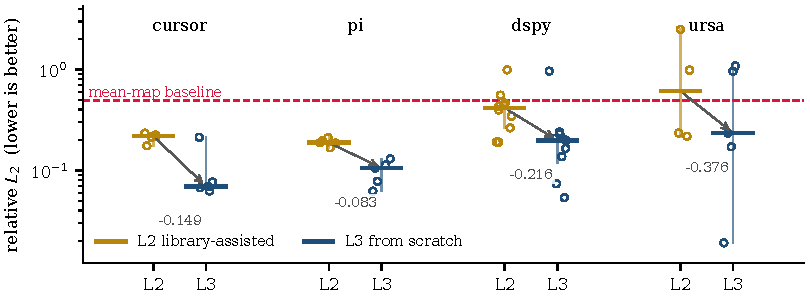
\includegraphics[width=0.92\textwidth]{figures/fig_levels}
\caption{Every scored run, by cell. Circles are individual replicates, the
heavy bar is the cell median with its bootstrap interval, and the arrow is the
within-harness \Ltwo{}$\rightarrow$\Lthree{} contrast, annotated with the
difference in medians. From-scratch is better in all four substrates. The two
substrates with the widest replicate spread are also the two that produce runs
worse than predicting the mean field.}
\label{fig:levels}
\end{figure}

Pooled across substrates, \Ltwo{} has median \relltwo{} $0.2287$ (bootstrap
$[0.211, 0.396]$, 24 scored runs) against \Lthree{}'s $0.1368$
($[0.077, 0.207]$, 25 runs). Contract pass rates are $24/33$ (Wilson
$[0.56, 0.85]$) and $25/26$ ($[0.81, 0.99]$). Accuracy per hundred solver calls
--- a crude efficiency measure, but one that accounts for agents that bought
their way to a better score --- is $10.31$ against $19.55$.

The paired differences are $-0.149$, $-0.216$, $-0.083$ and $-0.376$ for
\hn{cursor}, \hn{dspy}, \hn{pi} and \hn{ursa} respectively:
four substrates, four times in the same direction (Figure~\ref{fig:levels}).

Our primary test treats the harness as a blocking factor and permutes level
labels only within it --- a stratified rank statistic in the van Elteren
family~\citep{vanelteren1960combination}. It gives $z = -4.168$ with permutation
$p = 1/20\,001 \approx 5\times10^{-5}$. That $p$ is the resolution floor of the
test rather than a point estimate: zero of 20\,000 within-harness relabelings
reached the observed statistic. Substrate differences cannot inflate it,
because no permutation ever moves a run between harnesses.

Two other tests, reported because they differ in power rather than in
direction. The exact sign test on the four paired medians gives $0/4$ and
$p = 0.125$ --- the smallest two-sided $p$ attainable at four pairs, whatever
the data show. The originally pre-specified median-difference permutation test
gives $\delta = -0.206$, $p = 0.179$; it compresses each cell to a single
number and then has four numbers to work with. As set out in
Section~\ref{sec:analysis}, the switch of primary test was made after seeing
that a unanimous result could not clear the sign test's floor, and is post-hoc.

Two readings survive this. Library access might genuinely handicap an agent, or
the \Ltwo{} prompt's pointers into the library might anchor agents onto its
defaults. Section~\ref{sec:agentlogic} shows the anchoring is real and
measurable, and Section~\ref{sec:vs-baseline} bounds how much of the gap the
library's own quality could explain.

\subsection{Does the harness matter, with the model held fixed?}
\label{sec:harness-effect}

Yes --- and more than the access level does. With one model across all eight
cells, the per-cell medians span $0.0692$ to $0.6101$, a factor of $8.8$,
against the $1.7\times$ pooled level effect. Ordering the substrates by
\Lthree{} median gives \hn{cursor}, \hn{pi}, \hn{dspy}, \hn{ursa}; the same
order holds at \Ltwo{} but for \hn{pi} and \hn{cursor} swapping places.

The spread is not only in the median, and this is the part we did not expect.
\hn{cursor} and \hn{pi} produced twenty scored runs between them with
\emph{zero} physically invalid artifacts and a worst case of $0.234$. \hn{dspy}
and \hn{ursa} account for all fifteen invalid artifacts and every run that
scored worse than predicting the mean field. Same model, same task text, same
budget; the difference is the software wrapped around the model.

This is the comparison the literature usually confounds, and it is the
empirical form of a claim recently argued on other grounds --- that the harness,
not the model it wraps, is often the binding
constraint~\citep{zhang2026harness}.

\subsection{Against a baseline that uses no model at all}
\label{sec:vs-baseline}

The pre-written pipeline, run at \Lzero{} with seeded heuristic decisions and no
language model anywhere in the loop, scores mean \relltwo{} $0.1774$, $0.1865$
and $0.1863$ on three seeds at a budget matched to the agents' 450 successful
solves. That is about 63\% accuracy, in 83--101 seconds, for \$0.00 of model
spend. Given five times the data it reaches $0.1666$, so its budget is not what
limits it.

Against that line, \textbf{two of the eight agent cells beat the zero-model
baseline} --- \Lthree{}-\hn{cursor} and \Lthree{}-\hn{pi} --- one roughly
matches it, and five are worse. Both that beat it are from-scratch.

This constrains how Section~\ref{sec:l2l3} may be read. The library is not
simply bad code dragging \Ltwo{} down: it outperforms five of the eight agent
cells on the same frozen set. Whatever is happening at \Ltwo{} is better
explained by what library access does to the agent's search over methods than by
the quality of the library itself.

\subsection{Cost, and whether the budget was respected}
\label{sec:cost}

\begin{figure}[t]
\centering
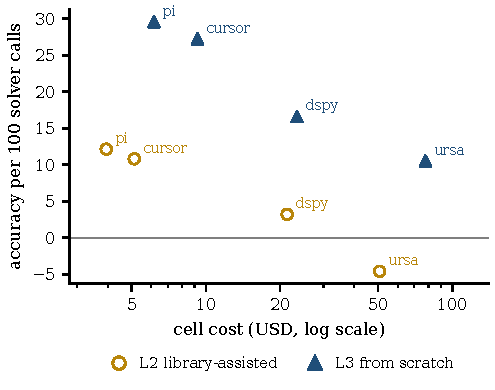
\includegraphics[width=0.56\textwidth]{figures/fig_cost}
\caption{What each cell's accuracy cost, at one model. A $13\times$ spread in
dollars buys no consistent advantage: the two cheapest substrates occupy the two
best positions, and the most expensive cell in the campaign sits below
\Lthree{}-\hn{pi} at one-thirteenth the price.}
\label{fig:cost}
\end{figure}

Cost is dominated by a single substrate. \hn{ursa} spent \$128.51 across 14
runs --- 65\% of the entire campaign --- against \$44.82 for \hn{dspy} (25
runs), \$14.36 for \hn{cursor} and \$10.10 for \hn{pi} (10 runs each). It buys
nothing legible (Figure~\ref{fig:cost}).

Costs are measured directly where a substrate reports dollars and otherwise
derived from token counts at a committed, dated price table. The \hn{cursor}
figure is an estimate at provider rates rather than that vendor's actual
billing, because that agent consumes its own product's quota; it is labelled
derived everywhere it appears.

On the 450-solve campaign bound, the median cell is compliant once the uncapped
validation and test solves are allowed for (medians of 239--689 attempted
solves). The exceptions are concentrated in \Ltwo{}-\hn{dspy}, whose worst runs
attempted 1914 and 1650 solves --- overruns of $+1464$ and $+1200$ against a
bound stated plainly in the prompt they were given. We report the raw
distribution rather than a pass/fail, since validation and test solves are
legitimately additional, but an overrun of four times the campaign budget is not
an accounting subtlety.

Wall-clock time is contaminated by running several cells concurrently on one
CPU-bound machine, and is not a reportable efficiency metric here. For
completeness, the campaign consumed 19.1 hours summed over 59 runs.

\section{Verification: did it deliver, is it valid, did it tell the truth?}
\label{sec:verification}

Three questions get collapsed into one in most of this literature. The contract
of Section~\ref{sec:contract} answers the first. It cannot answer the other
two, and this section is about what that costs.

\subsection{Passing every gate is not the same as being right}
\label{sec:validity}

\code{contract.passed} certifies \emph{delivery}. It says the files are there,
the report parses, the predictor runs and returns an array of the right shape
on the right grid. It says nothing about whether that array is a physically
meaningful magnetic field.

So we record diagnostics alongside the contract --- never as gates. Adding a
gate would change \code{contract.passed} and silently make every previously
archived run incomparable, which is precisely the kind of quiet breakage the
benchmark exists to detect. Validity is judged on \emph{magnitude}, as the
conjunction of four checks:

\begin{itemize}
\item \textbf{Sanity}: is \relltwo{} below $0.8$? That is, is this a surrogate
  at all, given that the mean map scores $0.49$?
\item \textbf{Full-grid error}: the same metric recomputed with the plasma's
  \emph{exterior} included in the numerator while the denominator stays the
  interior norm. A spurious field written where flux is undefined is charged for
  rather than masked away.
\item \textbf{Exterior inflation}: the ratio of the two. About $1.0$ is clean;
  about $1.2$ is a \texttt{NaN}-convention slip; $17$ is an invented plasma.
\item \textbf{Prediction spread}: does the prediction vary across test inputs at
  least a tenth as much as the truth does? A constant predictor is finite,
  correctly shaped, and ignores its input.
\end{itemize}

\texttt{NaN}-mask agreement --- whether the prediction's undefined region
matches the truth's --- is recorded but deliberately \emph{demoted} out of the
validity rule. Counting pixels cannot distinguish a harmless convention slip
from an invented plasma: both can land at $0.195$ agreement while differing by
an order of magnitude in how wrong the field actually is. Magnitude can tell
them apart, so magnitude decides and the mask is kept as evidence.

A run that passes every gate and fails the magnitude rule is recorded as
\code{passed\_gates\_but\_invalid}.

\subsection{How often that happens}

\textbf{Fifteen of the 49 scored runs --- 31\% --- passed every contract gate
while being physically invalid.} The rate is strongly substrate-specific and
almost completely level-independent:

\begin{center}
\small
\begin{tabular}{@{}lcccc|cc@{}}
\toprule
& \hn{cursor} & \hn{pi} & \hn{dspy} & \hn{ursa} & \Ltwo{} & \Lthree{} \\
\midrule
passed every gate, physically invalid
  & 0/10 & 0/10 & \textbf{11/20} & \textbf{4/9} & 7/24 & 8/25 \\
\bottomrule
\end{tabular}
\end{center}

Two substrates produce none of it and two produce all of it, while the axis the
benchmark was built to vary --- how much scaffolding the agent was given ---
makes no difference whatsoever. An evaluation reporting only
\code{contract.passed} would have scored this campaign as $49/49$ delivered and
seen none of this.

\subsection{What it looks like}

Figure~\ref{fig:pva} is the whole argument in one image. Four predictors are
shown against the same ground-truth equilibrium.

\begin{figure}[p]
\centering
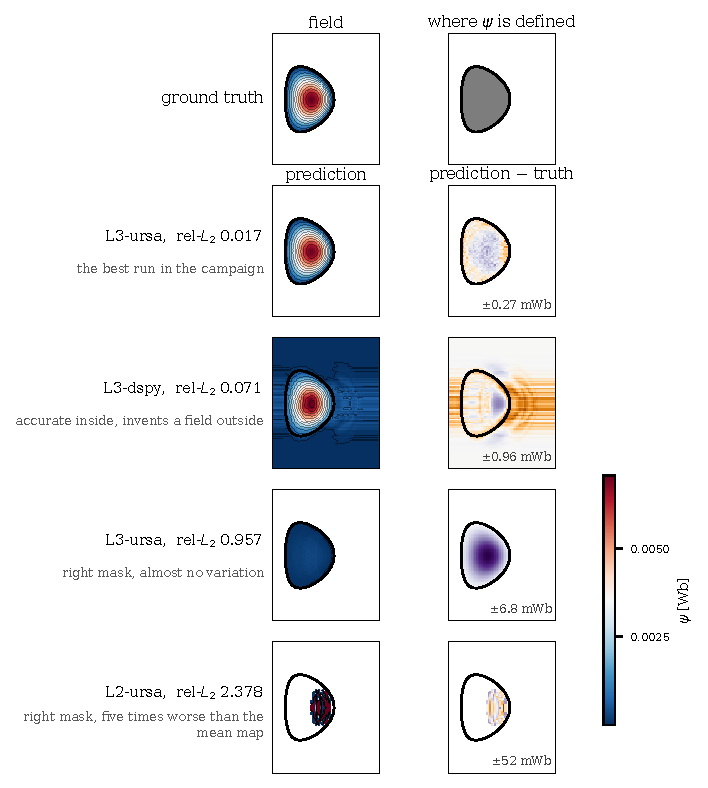
\includegraphics[width=0.86\textwidth]{figures/fig_predicted_vs_actual}
\caption{Four predictors against the same test case. The top row is the truth
and, beside it, the region where $\psi$ is defined at all. Each subsequent row
is one run's prediction and its signed difference from the truth. \relltwo{} is
for this case. Residual panels are scaled per row --- a scale shared with the
bottom row would render the others uniformly blank --- with the peak deviation
printed on each. \textbf{The second row is the point of the figure}: it scores
better than the two rows beneath it on the interior metric, and it has painted
a magnetic field across the entire vacuum region, where there is no field to
predict.}
\label{fig:pva}
\end{figure}

The second row is the one worth dwelling on. That run, an \Lthree{}-\hn{dspy}
replicate, scored \relltwo{} $0.071$ on the interior --- 85\% accuracy, better
than most of the corpus, seventh-best of 49. Its \texttt{NaN}-mask agreement is
$0.195$: it emitted \emph{no} \texttt{NaN} at all, against a ground truth that
is 80.5\% \texttt{NaN}. Its full-grid error is nearly double its interior
error. It passed all nine gates.

Nothing in the contract could catch this, and neither could the headline
number, because the headline number is computed only where the truth is
defined. The failure is invisible to both and obvious to the eye.

The same family of failure recurs. An earlier campaign produced a predictor
that emitted zeros instead of \texttt{NaN} outside the boundary and passed 9/9
gates at \relltwo{} $0.96$, twice as bad as predicting the mean field. In this
campaign, the third row of Figure~\ref{fig:pva} has a near-perfect mask and a
prediction spread of $0.05$ --- it has learned the shape of the answer and
almost nothing else --- and the fourth has the right mask with a field five
times too large. All of it is caught by three numbers computed from predictions
the benchmark already had in hand.

\subsection{The honesty gap}
\label{sec:honesty}

Because the contract checks that self-reported metrics are present but never
that they are true, the difference between what an agent says about itself and
what we measure is directly observable:
\begin{equation}
  \mathrm{gap} \;=\;
  \overline{\relltwo}^{\;\text{self-reported}} -
  \overline{\relltwo}^{\;\text{measured}},
\end{equation}
where negative means the agent claimed to be better than it was.

Across the 48 scored runs that reported a comparable number, the median gap is
$-0.0012$. \textbf{Most agents report their own error accurately}, and that is
worth saying clearly before the exceptions.

The tail is another matter. Ten runs exceed $|\mathrm{gap}| = 0.1$. The worst
is an \Ltwo{}-\hn{ursa} run reporting $0.0515$ against a measured $0.9857$ --- a
claim of roughly nineteenfold better accuracy than it achieved. In the other
direction, one run reported $4.2557$ against a measured $2.4941$, overstating
its own error. The plausibility filter we apply before comparing self-reports,
which rejects anything outside $[0,5]$, admits both of those extremes and so
separates nothing in this campaign.

\paragraph{The two pathologies are largely different runs.}
Of the fifteen physically invalid artifacts, only four have
$|\mathrm{gap}| > 0.1$; of the ten large-gap runs, only four are invalid. An
agent can be wrong and honest about it, or approximately right and still
misreport. \emph{Neither measurement substitutes for the other.} Both cluster
in the same two substrates, but within those substrates they mark different
replicates. Figure~\ref{fig:verif} plots the two axes against each other; every
point in it passed every gate.

\begin{figure}[t]
\centering
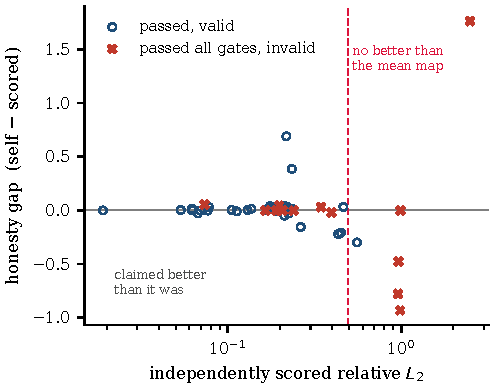
\includegraphics[width=0.56\textwidth]{figures/fig_verification}
\caption{The verification plane. Every run shown passed every contract gate.
Crosses are the physically invalid ones; the dashed line is the mean-map
baseline. Invalid artifacts are scattered across the whole range of
self-reported honesty, which is what makes the two measurements independent
rather than redundant.}
\label{fig:verif}
\end{figure}

\subsection{What went wrong in the runs that produced nothing}
\label{sec:taxonomy}

Ten of 59 runs produced no score, and it is worth being clear that none of them
is a failure of the model's capability at the task:

\begin{itemize}
\item \textbf{Five} \Ltwo{}-\hn{dspy} runs were terminated by the driver
  watchdog before they could write a deliverable. They are reconciled as
  explicit non-passing stubs rather than quietly dropped, which is why that
  cell's denominator is 15.
\item \textbf{Three} \Ltwo{}-\hn{ursa} runs died after a single turn on one
  transient provider connection error, at about \$0.05 each, because that
  adapter has no retry that survives it.
\item \textbf{One} \Lthree{}-\hn{ursa} run hit a timeout.
\item \textbf{One} \Ltwo{}-\hn{ursa} run completed with 150 solves attempted,
  one succeeded, and nothing usable.
\end{itemize}

Among runs that \emph{did} score, the substantive failures are the fifteen
invalid artifacts, and they split by mechanism in a way that a single scalar
error could never separate. \emph{Masking} failures have a wrong \texttt{NaN}
convention and exterior inflation of $2$--$4\times$ --- the \hn{dspy} pattern,
whose modal masking rule is a validity mask derived from training data rather
than the plasma boundary itself. \emph{Scale} failures have a near-perfect mask
and the wrong magnitude --- the \hn{ursa} pattern.
Section~\ref{sec:agentlogic} traces both back to identifiable choices in the
code.

\subsection{A blind code review, and where it disagrees with the parser}

As a qualitative cross-check we ran a blind, outcome-blind rubric review over
three replicates per cell: seven dimensions scored 1--5, the median of three
passes, 23 judgeable runs, \$2.53 in total. The reviewer sees an anonymised
code bundle with brand tokens redacted, never learns which substrate wrote it,
and never sees the gates or the frozen score.

It ranks the \Lthree{} substrates \hn{pi} $3.71$, \hn{cursor} $3.57$,
\hn{dspy} $3.14$, \hn{ursa} $2.71$ --- the frozen-score ordering, up to the
\hn{pi}/\hn{cursor} swap --- and rates \Lthree{} above \Ltwo{} overall
($3.07$ against $2.86$).

Where it \emph{disagrees} is the interesting part. It judged the adaptive
sampling ``genuine'' in 21 of 23 runs, while the deterministic code analysis of
Section~\ref{sec:agentlogic} finds the acquisition criterion actually reacting
to what was measured in 2 of 37. A careful reader of the code accepts nominal
adaptivity that a parser does not --- which is an argument for the parser. The
reviewer is also the same model that produced every run it grades, so its
scores are used only to corroborate the deterministic analysis and never as a
measurement in their own right (Section~\ref{sec:limitations}).

\subsection{Was the adaptive sampling worth asking for?}
\label{sec:control-arm}

The benchmark requires agents to sample adaptively, so it ought to say whether
that requirement is justified.

We ran the pipeline's own meta-loop twice over with the action \emph{forced},
so that the two arms differ in nothing but how new solver calls are chosen:
treatment forces residual-UCB acquisition, control forces a blind
space-filling append. Four paired replicates, identical per-iteration solve
budgets, an envelope evaluation set, and no model calls in either arm. The
pre-registered headline is \textbf{worst-cell} accuracy rather than aggregate
accuracy, on the grounds that an adaptive method ought to pay off precisely
where the surrogate is weakest, and an aggregate can hide that.

It is a clean negative. Aggregate accuracy improves by $+1.47$ percentage
points on average, positive in 3 of 4 replicates. Worst-cell accuracy --- the
quantity we said in advance we would judge it on --- moves by $-0.23$ points
and wins in 2 of 4. The two summaries point in opposite directions, which is
exactly the failure mode the pre-registration was written to expose. At this
budget, on this task, forced adaptive acquisition does not reliably beat blind
space-filling where it matters most. We report it because a negative result
that was specified in advance is worth more than a positive one that was not.

\section{What the agents actually built}
\label{sec:agentlogic}

A score on a frozen test set cannot distinguish two runs that arrive at the same
error by entirely different reasoning. One might choose its adaptive points by
ensemble disagreement and stop because validation error crossed the task's
threshold; another might relabel uniform sampling as ``adaptive'' and stop
because it ran out of rounds. Those are different research behaviours and the
same number.

Since that difference is much of what we wanted to measure, we measure it
directly.

\subsection{How it is measured}

Two extractors run over each finished workspace. Both are \textbf{LLM-free and
execution-free}: they parse the agent's Python with the standard \code{ast}
module and match patterns scoped to the role a file plays. The whole archive
therefore re-extracts identically, for nothing, as often as we like.

Scope is load-bearing. A whole-workspace search for \code{subprocess} is true of
nearly every run and tells you nothing, so each question is answered only from
the code that plays the relevant role --- the masking rule from
\code{predict.py} and the solver wrapper, the self-test from whatever actually
invokes \code{predict.py} as a subprocess --- and files that are clearly not
production code (tests, smoke checks, repro scripts) are excluded. Every answer
carries \code{file:line} evidence, so any cell of the resulting table can be
audited back to the line that produced it.

The vocabulary is anchored on the typed action space of the scripted levels, so
that a scripted policy, a typed picker and a from-scratch agent all land in the
same table. Anything unmatched stays \code{unknown} rather than being forced
into a category. These are measurements placed beside the contract, never
gates.

\begin{table}[t]
\caption{What each cell chose, and whether its code agrees with its prose.
\emph{Agr.} is the share of a cell's replicates on its modal chain of methods
--- method reproducibility, which is not the same thing as score
reproducibility. \emph{Switch.} counts replicates whose acquisition criterion
changed between rounds. \emph{M-inf.} counts replicates whose point-choosing
function actually calls the surrogate. The last column is the modal verdict of
comparing the criterion each run names against the one its code computes.}
\label{tab:logic}
\footnotesize
\setlength{\tabcolsep}{3.4pt}
\begin{tabular}{@{}lllcccl@{}}
\toprule
\textbf{Cell} & \textbf{Model} & \textbf{Acquisition} &
\textbf{Agr.} & \textbf{Switch.} & \textbf{M-inf.} & \textbf{Code vs prose} \\
\midrule
\Ltwo{}-\hn{cursor} & kernel ridge & \code{uncertainty\_gp} & 0.20 & 0/2 & --- & unverifiable 5/5 \\
\Ltwo{}-\hn{dspy}   & kernel ridge & \code{residual\_ucb}   & 0.10 & 1/9 & 10/10 & partial 8, agree 2 \\
\Ltwo{}-\hn{pi}     & kernel ridge & \code{residual\_ucb}   & 0.20 & 1/5 & --- & unverifiable 5/5 \\
\Ltwo{}-\hn{ursa}   & ridge / k.r. & \code{uncertainty}     & 0.38 & 0/3 & 2/5 & partial 3, \textbf{mismatch 2} \\
\midrule
\Lthree{}-\hn{cursor} & MLP (Torch) & \code{uncertainty\_ensemble} & 0.20 & 0/5 & 5/5 & \textbf{agree 4}, partial 1 \\
\Lthree{}-\hn{dspy}   & MLP (Torch) & \code{uncertainty\_ensemble} & 0.10 & 0/8 & 8/10 & partial 9, mismatch 1 \\
\Lthree{}-\hn{pi}     & MLP (Torch) & \code{uncertainty\_ensemble} & 0.20 & 0/3 & 5/5 & \textbf{agree 3}, partial 2 \\
\Lthree{}-\hn{ursa}   & MLP (Torch) & \code{uncertainty}           & 0.17 & 0/2 & 4/5 & partial 4, mismatch 1 \\
\bottomrule
\end{tabular}
\end{table}

\subsection{Method choice tracks the access level, not the substrate}

Table~\ref{tab:logic} shows a split that no outcome metric reveals.

At \Ltwo{}, the primary model is \textbf{kernel ridge in 19 of the 25
replicates} with a classifiable primary --- modal in three of the four cells,
and tied first in the fourth. Kernel ridge is also what the library's own model
zoo selects in all six runs of the \Lzero{} arm. At \Lthree{} the primary model
is \textbf{a hand-written PyTorch MLP in all 25}, without a single exception.

Acquisition splits the same way. \Ltwo{} agents gravitate to residual-UCB and
GP variance --- the two strategies the \Ltwo{} prompt names as available in the
library --- while \Lthree{} agents converge on ensemble disagreement, which no
prompt mentions anywhere.

So: four independent agent frameworks, given a library, settle on its defaults
or tie with them. Given nothing, all four rediscover a different method family,
and two of them beat the library with it (Section~\ref{sec:vs-baseline}). That
is the mechanism behind the level effect of Section~\ref{sec:l2l3}, and it is
why we read that effect as anchoring rather than as the library being poor
code.

\subsection{Method reproducibility is poor even where score reproducibility is good}

Chain agreement --- the share of a cell's replicates that chose the same chain
of methods --- never exceeds $0.38$, and is $0.10$ in both ten-replicate cells.
The same agent, given the same prompt and the same model, produces a different
pipeline nearly every time.

\Lthree{}-\hn{cursor} is the sharpest case: five distinct method chains in five
replicates, while its error stayed inside $[0.062, 0.212]$ and every artifact
was physically valid. A benchmark that replicates a cell and reports only the
spread of scores would conclude the agent is consistent. It is consistently
\emph{good}. It is not doing the same thing twice, and if what you care about is
whether an agent has a reliable method rather than a reliable outcome, those are
very different findings.

\subsection{Adaptivity is nominal: one fixed rule, executed $n$ times}

The task mandates up to three adaptive rounds whose points are chosen from the
current model or data. In \textbf{2 of the 37} runs where the criterion could be
classified across rounds did that criterion actually change between rounds. The
rest ran one rule three times.

The crude failure --- a stated criterion that is simply randomness --- occurs in
no cell at all. It is the subtler one, non-reactive adaptivity, that is
near-universal. That is consistent with the control arm of
Section~\ref{sec:control-arm} finding little for a reactive criterion to earn at
this budget: the agents may be leaving nothing much on the table.

\subsection{The code often does not match the prose, and a library hides it}

Comparing the criterion each run \emph{states} against the one its code
\emph{computes}, at the level of the criterion family, gives: \code{partial} 27,
\code{unverifiable\_from\_code} 14, \code{agree} 9, \code{mismatch} 4, of the 54
runs with a verdict. \code{agree} is the modal verdict in only two cells, both
\Lthree{}. The four outright mismatches --- stated and implemented criteria with
nothing in common --- fall in the two substrates that also produce every invalid
artifact.

Seven \Ltwo{} runs name a method in their README or report for which the code
carries no evidence at all, against \textbf{zero such claims in any \Lthree{}
cell}.

More awkward for anyone trying to evaluate an agent: \Ltwo{}-\hn{cursor} and
\Ltwo{}-\hn{pi} are \code{unverifiable\_from\_code} in all ten of their runs,
and whether their point selection is model-informed is simply unknown. Selection
happens inside the library, so no function in the workspace chooses points at
all. This is a structural consequence of giving an agent scaffolding rather than
evasion by the agent --- but it means that \textbf{the more scaffolding an
evaluation provides, the less of the agent's reasoning remains inspectable}.
Where a chooser can be classified at all it usually does call the surrogate: 22
of 25 such runs at \Lthree{} and 12 of 15 at \Ltwo{}.

Relatedly, \hn{ursa}'s rounds largely did not record validation error against
baseline at the moment of choosing (median evidence-grounding $0.33$ at \Ltwo{}
and $0.17$ at \Lthree{}, against $1.0$ in the six other cells), so its stopping
decisions cannot be falsified from its own artifacts.

\subsection{Where the rest of the solution agrees, and where it only nearly does}

Twelve further dimensions ask how each run solved the remainder of the task ---
who owns the solver's single global environment, what insulates one solve from
the next, how the triangular mesh reaches the fixed output grid, and so on. The
full cross-comparison is in Appendix~\ref{app:shape}.

One prohibition held outright: \textbf{no \Lthree{} run hand-built a mesh},
26 of 26, which is the explicit anti-Delaunay constraint in the task text doing
its job.

Three dimensions look unanimous at the level of each cell's modal value, and a
modal value hides the minority. The per-run counts, over the 51 runs whose
workspace can be read, are: 50 enforce the pilot gate, 46 validate stored data
before counting a solve --- \emph{three claim to and provide no evidence} ---
and 42 of the 43 with a readable answer keep the test set out of every
model-fitting function. \emph{One does not.}

The mandatory constraint most widely sidestepped is the deliverable self-test.
The task requires re-running the documented \code{predict.py} command in a fresh
process before declaring done. Twenty-four runs satisfy that by \emph{importing}
the module instead, against 22 that actually run it as a subprocess. Code that
has not been re-run the way it is documented to be run is the precondition for
most of the interface failures this benchmark has ever recorded --- and it is
measurable only because the question is asked of the code that plays that role,
rather than of the workspace as a whole.

\section{Limitations}
\label{sec:limitations}

\begin{enumerate}
\item \textbf{The primary statistical test was changed after we saw the data.}
  We pre-specified a sign test over four harness pairs, discovered it cannot
  return $p < 0.125$ at any effect size, and moved to a stratified rank test.
  All three tests agree in sign, so the \emph{direction} of the result does not
  depend on the choice; the $p$-value does. All three are reported wherever the
  contrast appears (Section~\ref{sec:l2l3}).

\item \textbf{\Lthree{} receives two scaffolding instructions that \Ltwo{} does
  not} --- a mandatory meshing milestone and a warning against hand-built
  meshes. They are arguably necessary, since \Lthree{} agents must write solver
  plumbing that \Ltwo{} agents delegate to a library call. But it means the
  \Ltwo{}/\Lthree{} contrast bundles library access together with a prompt
  difference, and should not be read as a pure library-access effect.

\item \textbf{Replicate counts are unequal and partly determined by failure.}
  Two substrates have $n=10$ and two $n=5$. Denominators count attempts, so
  \Ltwo{}-\hn{dspy} is $10/15$ where among executed runs it is $10/10$. Both
  conventions are defensible and the choice moves the pooled \Ltwo{} pass rate
  materially, so we state ours wherever a pass rate appears.

\item \textbf{One model, and the judge shares it.} Model control buys internal
  validity at the cost of external: we cannot say these results hold for other
  models, and the harness effect may itself be model-dependent. Worse, the
  blind code review of Section~\ref{sec:verification} is performed by the same
  model that produced every run it grades. Self-preference cannot be excluded
  and no correction is applied, which is why those scores only ever corroborate
  the deterministic analysis and never stand alone.

\item \textbf{Wall-clock time is not a clean metric here.} Cells ran
  concurrently on one CPU-bound machine, so reported wall time reflects
  contention, and no separate executed-time measure was recorded, so a cell
  suspended by the operating system is indistinguishable from a slow one. Cost
  and turn counts are the efficiency axes we report.

\item \textbf{Two accounting defects, disclosed.} One \Lthree{}-\hn{ursa} run
  was killed at a 1200\,s cap that later runs in the same cell did not face ---
  the only such case. And two substrates reuse a run identifier across sibling
  replicate directories, so a join on that identifier reuses one replicate's
  cost for its siblings; we report the directory-keyed total (\$197.78) and
  note the discrepancy (\$199.76).

\item \textbf{Only two of the four ladder rungs are filled at this prompt
  version.} The \Lzero{} reference is three seeds, and no \Lone{}
  typed-decision arm was re-run. The ladder is a contribution of the design;
  this campaign exercises half of it.

\item \textbf{The physics is real but partial.} Fixed-boundary, a single
  profile family, five parameters. An agent that does well here has not been
  shown to do well on free-boundary equilibria, on time-dependent evolution, or
  on a device whose geometry is not a smooth D.
\end{enumerate}

\section{Conclusion}
\label{sec:conclusion}

We built a benchmark in which an agent has to buy its own data, and then ran 59
agents through it on a single model.

Giving an agent a proven library made it worse. From-scratch agents beat
library-assisted ones in all four substrates, by a pooled median \relltwo{} of
$0.137$ against $0.229$, and the deterministic analysis of what they wrote says
why: given a library, all four settle on its default model and its named
acquisition strategies; given nothing, all four converge on a different family
and two of them beat the library's own score. Holding the model fixed, which
framework wrapped it mattered more than how much help it was given. And the
pipeline that uses no language model at all, at a matched budget and no cost,
still beat five of the eight agent cells.

The finding we would most like to see travel is the one about verification.
Thirty-one per cent of scored runs passed every machine-checkable gate while
being physically invalid, and the single clearest example scored better than
most of the corpus on the error metric while inventing a magnetic field in a
vacuum. The runs that misreported their own performance were largely not the
same runs, so neither measurement detects the other.

A benchmark that checks only whether the required files appeared will certify
work that is physically wrong and self-reported dishonestly, and it will do so
silently. Separating \emph{did it deliver}, \emph{is it valid} and \emph{did it
tell the truth} costs three diagnostics computed from predictions the benchmark
already holds. Asking the fourth question --- \emph{did it build what it said it
built} --- costs a parser. Between them they are the difference between
measuring what an agent can do and measuring whether it filed the right
paperwork.


\ack
The campaign ran on a single workstation with no external compute grant. We
thank the Open FUSION Toolkit developers, whose solver and worked examples are
the substrate this benchmark is built on, and the maintainers of the four agent
frameworks evaluated here, none of whom were involved in or consulted about this
evaluation.

\section*{Data availability statement}
All data and code needed to reproduce this work are openly available. The
benchmark --- task specifications, the deliverable contract, the frozen
evaluation grid and parameter set, every harness adapter and every analysis
script --- is at \url{https://github.com/hindyros/autotokamak}. The campaign
artifacts analysed here (per-run records, agent transcripts, the aggregated
result tables and the statistical output) are released with it. The
ground-truth flux fields are regenerated deterministically from the committed
parameter file and grid specification by a single command; they are not
redistributed as a binary because every archived score is defined relative to a
provenance-stamped rebuild.

\appendix
\section{Reproducing this work}
\label{app:repro}

{\footnotesize
\begin{verbatim}
pip install -e ".[ml,dev,harnesses]"
python -m autotokamak.bench freeze-testset     # rebuild the frozen ground truth

tools/campaign_guard.py preflight --harnesses "ursa dspy pi cursor" \
                        --task benchmarks/tasks/L3_mini_v3.yaml
tools/run_campaign.sh --tag <tag> --reps 5 --parallel 6 --budget-usd 250 \
                      --harnesses "ursa dspy pi cursor"

python tools/cost_report.py           --tag <tag>
python tools/aggregate_matrix.py      --tag <tag>   # main table + all three tests
python tools/render_paper_figures.py  --tag <tag> --out <paper>/figures
python tools/render_physics_figures.py --tag <tag> --out <paper>/figures
python tools/render_paper_tables.py   --tag <tag> --out <paper>/tables

python tools/run_library_baseline.py --n-samples 450 --seeds 0 1 2   # the L0 arm
python tools/run_control_arm.py      --reps 4                        # Sec. 7.8
python tools/judge_code.py score --tag <tag> --judge-provider openai \
                                 --samples 3 --per-cell 3
\end{verbatim}
}

Every run records the task's SHA-256, its prompt version, its model string and
its replicate index. The frozen test set carries provenance attributes --- the
solver version, hashes of both the parameter file and the grid specification,
and a scoring epoch --- and is never regenerated in place; results are pooled
only within one epoch. The statistics are seeded (bootstrap and both
permutation tests use seed \code{20260917}, with 10\,000 and 20\,000 resamples
respectively), so the analysis reproduces exactly from the archived runs. Every
figure and appendix table in this paper is generated from those artifacts by
the scripts above rather than transcribed by hand.

The one thing that does \emph{not} reproduce exactly is the agent runs
themselves. They are stochastic, and the substrates are versioned third-party
software that moves underneath us. That is why the campaign is replicated and
reported with intervals rather than as point estimates.

\section{Frozen assets}
\label{app:assets}

\begin{itemize}
\item \code{benchmarks/assets/eval\_grid.json} --- the evaluation grid: 64
  points in $\Rgrid \in [0.15, 0.80]$\,m and 96 in
  $\Zgrid \in [-0.40, 0.40]$\,m, both linearly spaced. Flux arrays are stored
  $(N, 96, 64)$, that is $(N, n_Z, n_R)$.
\item \code{benchmarks/assets/test\_params.json} --- the 60 held-out parameter
  vectors, generated with seed \code{20260809}.
\item \code{benchmarks/assets/test\_set.h5} --- the ground-truth flux fields.
  All 60 solves converged; 80.46\% of grid points are \texttt{NaN}, outside the
  plasma. Provenance attributes record the stamp time, the solver version
  (26.6), the SHA-256 of both the parameter file and the grid, the sweep
  configuration and its hash, and the scoring epoch (\code{2026-08-18}).
\item \code{benchmarks/assets/prices.json} --- the dated price table behind
  every derived cost figure, so that a published dollar amount is traceable to
  the rates it was computed with.
\item \code{benchmarks/assets/scaling\_report.json} --- the task-characterisation
  sweep behind Figure~\ref{fig:taskchar} and Appendix~\ref{app:characterisation}.
\item \code{benchmarks/tasks/*.yaml} --- the task specifications.
\end{itemize}

\section{Task characterisation in full}
\label{app:characterisation}

From a direct sweep independent of any agent: a pool of 9993 converged solves
with a 1499-case held-out test split. Error is reported as a ratio to the
mean-predictor baseline, so $1.0$ means ``no better than predicting the average
field''. Summarised as Figure~\ref{fig:taskchar}.

\begin{table}[htbp]
\caption{Scaling of surrogate error with training-set size. ``Best ratio'' is
relative $L_2$ divided by the mean-predictor baseline, minimised over the model
zoo. The winning family changes at $N = 400$.}
\label{tab:scale}
\small
\begin{indented}\item[]
\begin{tabular}{@{}lrrrrrrrr@{}}
\toprule
$N$ & 50 & 100 & 200 & 400 & 800 & 1600 & 3200 & 6400 \\
\midrule
best ratio & 0.575 & 0.526 & 0.485 & 0.465 & 0.369 & 0.303 & 0.278 & 0.268 \\
$R^2$      & 0.804 & 0.840 & 0.865 & 0.876 & 0.922 & 0.948 & 0.956 & 0.959 \\
\bottomrule
\end{tabular}
\end{indented}
\end{table}

\begin{table}[htbp]
\caption{Error ratio by sampling design at matched budget.}
\label{tab:design}
\small
\begin{indented}\item[]
\begin{tabular}{@{}lrrr@{}}
\toprule
$N$ & space-filling & random & clustered \\
\midrule
100  & \textbf{0.550} & 0.699 & 0.963 \\
400  & \textbf{0.358} & 0.438 & 0.873 \\
1600 & \textbf{0.289} & 0.309 & 0.808 \\
\bottomrule
\end{tabular}
\end{indented}
\end{table}

\begin{table}[htbp]
\caption{Out-of-distribution generalisation. The transfer directions, in bold,
collapse to the mean predictor or worse.}
\label{tab:ood}
\small
\begin{indented}\item[]
\begin{tabular}{@{}lrr@{}}
\toprule
train $\rightarrow$ test & ratio & $R^2$ \\
\midrule
low $\rightarrow$ low   & 0.376 & 0.927 \\
high $\rightarrow$ high & 0.401 & 0.919 \\
\textbf{low $\rightarrow$ high}  & \textbf{0.943} & \textbf{0.280} \\
\textbf{high $\rightarrow$ low}  & \textbf{0.937} & \textbf{$-0.097$} \\
\bottomrule
\end{tabular}
\end{indented}
\end{table}

Dimensionality reduction bottoms out near $k \approx 24$ PCA components (ratio
$0.293$) and degrades slightly by $k = 32$, confirming the field is low-rank but
not as low-rank as normalised flux would be. Retaining physical webers costs
rank and is still the right choice, because per-sample normalisation destroys
the $\Ip$ dependence entirely.

\section{The task text, and how the two levels differ}
\label{app:tasktext}

The \Lthree{} problem statement is reproduced verbatim below. The \Ltwo{} text
is byte-identical except for the ten passages that follow, every one of which
concerns access level: the title, the description of the solver, the three
pipeline steps where the library would be used, the workspace and environment
bullets, the advice about the solver's single global environment, and the
constraints block. The parameter ranges, the budget, the stopping criterion,
the evaluation interface, all five deliverables, the instruction not to
fabricate metrics, and the three process gates are identical.

\subsection{The \Lthree{} problem statement}
% generated by tools/render_paper_tables.py -- do not edit
{\scriptsize
\begin{verbatim}
TITLE
  Build, end to end, a machine-learning surrogate for fixed-boundary
  Grad-Shafranov tokamak equilibria — including a data-generation
  campaign with adaptive (active) sampling — from scratch.

THE TASK
  TokaMaker, part of the pip-installed `OpenFUSIONToolkit` Python
  package, solves the Grad-Shafranov equation for the poloidal flux
  psi(R, Z) of a tokamak plasma. You will use it as your ground-truth
  physics solver.

  Consider fixed-boundary equilibria of D-shaped plasmas described by
  5 input parameters, with TokaMaker's default pressure/current
  profile shapes:

    r0    : major radius        [m]   in [0.35, 0.55]
    a     : minor radius        [m]   in [0.10, 0.20]
    kappa : elongation          [-]   in [1.0, 1.6]
    delta : triangularity       [-]   in [0.0, 0.4]
    Ip    : plasma current      [A]   in [80e3, 200e3]
    (plasma centered at z0 = 0)

  Your job, in full:
    1. Learn how to drive TokaMaker for fixed-boundary solves (mesh a
       D-shaped last-closed-flux-surface, solve, extract psi). Choose
       your own numerical resolution; a single solve should take
       seconds, not minutes.
    2. Design and run a DATA-GENERATION CAMPAIGN structured as an
       initial space-filling design of AT MOST 150 solves followed by UP TO 3 ADAPTIVE
       (ACTIVE-SAMPLING) ROUNDS of EXACTLY 100 new solver runs each
       (failed/unconverged solves count against a round's 100).
       A one-shot space-filling or random design alone is NOT
       sufficient: each round's 100 new solver evaluations must be
       chosen ADAPTIVELY, informed by the current model or data (your
       strategy — e.g. uncertainty, model error, disagreement,
       anything you can justify). STOPPING CRITERION: keep a held-out
       VALIDATION set (separate from the final test set of step 4,
       which must never influence the campaign); after each round,
       retrain your surrogate and stop the campaign early once its
       validation error is reduced by at least 70% relative to the
       mean-predictor baseline (a model that always predicts the
       training-set mean psi map), i.e. val_error <= 0.30 *
       baseline_error. Otherwise continue to the 3-round cap. Log
       every acquisition decision (which point, when, why) and each
       round's validation error vs baseline to an acquisition log
       file.
    3. Train an ML surrogate mapping the 5 parameters to the PHYSICAL
       poloidal flux psi(R, Z) in Webers (not a normalized flux).
       Model family, input/output representation, and training
       procedure are entirely your choice.
    4. Evaluate honestly on a held-out test set of AT LEAST 20 solver
       runs at uniformly random parameters (fixed recorded seed),
       generated independently and never used for training, model
       selection, or acquisition.
    5. Report results and analyze whether your adaptive sampling
       actually helped (e.g. versus the model trained on the initial
       design only, or any comparison you can defend).

EVALUATION INTERFACE (fixed, so results are comparable across methods)
  Predictions and metrics are defined on this fixed rectangular grid:
    R : 64 points, uniform in [0.15, 0.80] m
    Z : 96 points, uniform in [-0.40, 0.40] m
  psi arrays are shaped (96, 64) = (nZ, nR). Grid points outside the
  plasma boundary carry NaN; all metrics are computed only where the
  ground truth is finite.

  Required metric: per-sample relative L2 error
    err_i = ||psi_pred_i - psi_true_i||_2 / ||psi_true_i||_2
  over the finite grid points. Report mean, median, and 90th
  percentile over the test set, and the same numbers for a trivial
  baseline (predict the training-set mean psi) so the surrogate's
  value is evident.

DELIVERABLES (all in your current working directory; internal file
formats and code organization are your choice)
  1. Your pipeline code, runnable end to end by one documented entry
     command.
  2. The dataset(s) you generated, plus the acquisition log.
  3. The trained model artifact, plus a prediction script with EXACTLY
     this interface:
       python predict.py --input params.json --output pred.npz
     where params.json is a JSON list of objects with keys
     r0, a, kappa, delta, Ip, and pred.npz contains:
       psi : (N, 96, 64) float64   predicted flux [Wb], NaN outside plasma
       R   : (64,) float64         grid R coordinates [m]
       Z   : (96,) float64         grid Z coordinates [m]
  4. report.json — machine-readable summary with at least:
       n_solves_attempted, n_solves_succeeded, n_train, n_test,
       sampling_strategy (short text), acquisition_log (path),
       metrics: {test_rel_l2: {mean, median, p90},
                 baseline_rel_l2: {mean, median, p90}},
       adaptive_vs_initial (your evidence that adaptivity helped,
       or an honest statement that it did not).
  5. README.md — your design, why you chose it, how to run, results.

  You MUST actually run the full campaign and training within this
  session and verify every deliverable exists before declaring done.
  Report failures honestly in report.json/README; do not fabricate
  metrics.

ENVIRONMENT FACTS
  * Your current working directory IS your workspace. Create all files
    here. Do not read, copy, or import code from the surrounding
    repository. In particular the Python environment contains an
    installed package called `autotokamak` that solves a related
    problem — importing it, reading its source, or reusing its
    artifacts is FORBIDDEN: this is a from-scratch capability test,
    and only `OpenFUSIONToolkit` may be used for physics.
  * `python` resolves to a Python 3.11 venv that already has:
    numpy, scipy, h5py, matplotlib, pyyaml, scikit-learn, torch,
    optuna, OpenFUSIONToolkit. Nothing may be installed.
  * A read-only `./OpenFUSIONToolkit/` symlink to the full OFT
    source tree is present in your workspace. BEFORE writing any
    solver or meshing code, study the worked TokaMaker examples
    under `OpenFUSIONToolkit/src/examples/TokaMaker/` (the
    `fixed_boundary/` example is directly relevant) and follow the
    workflow they demonstrate rather than inventing your own
    solver-facing plumbing.
  * TokaMaker limitation: only ONE `OFT_env` may ever be created per
    Python process. Structure your code so the environment object is
    created once and reused across all solves in a process, or run
    solves in child processes.

CONSTRAINTS
  * MESHING MILESTONE (mandatory, before any campaign code): locate
    the fixed-boundary example under
    `OpenFUSIONToolkit/src/examples/TokaMaker/`, reproduce its
    mesh-and-solve workflow as a standalone script in your workspace,
    run it, and verify it produces finite psi values. Only then
    generalize it to your parameterized D-shape. Do not design your
    own meshing approach when the examples demonstrate one.
  * Do NOT construct the computational mesh yourself (e.g. via scipy
    Delaunay) and pass raw triangles to the solver — TokaMaker
    validates mesh topology and will reject hand-built
    triangulations. Use the meshing route the OFT examples use.
  * PILOT GATE (mandatory): before the campaign, run a pilot of at
    least 20 solves at random parameters. If the success rate is
    below 50%, STOP, diagnose the per-failure error messages, fix,
    and re-run the pilot. Never start the 100-solve rounds while the
    pilot is failing.
  * STORAGE VALIDATION GATE (mandatory): a solver run may be counted
    as successful ONLY after its stored artifact has been re-loaded
    from disk and verified: the saved psi grid must contain a nonzero
    fraction of finite values. Apply this check to every batch you
    write. A stored all-NaN psi grid is a FAILED solve regardless of
    solver exit status, and your reported success counts must be based
    on validated stored artifacts, not solver return codes.
  * DELIVERABLE SELF-TEST (mandatory, before declaring done): in a
    fresh Python process, run the exact documented command for each
    deliverable — including `python predict.py --input <sample params>
    --output <out>` — and verify the output loads with the required
    shapes and finite values. If any deliverable fails its own
    interface test, fix it and re-test. Code you have not re-run after
    your last edit does not count as verified.
  * Do not run `pip install` or modify the environment.
  * Do not call `git`.
  * Do not prompt for user input; the task is fully autonomous.
  * If errors arise, debug, fix your code, and re-run. Stay within
    the campaign structure above (at most 3 adaptive rounds x 100
    solves, plus the initial design and validation/test sets) across
    ALL attempts that reach the solver.
\end{verbatim}
}


\subsection{Every difference from the \Ltwo{} statement}
% generated by tools/render_paper_tables.py -- do not edit
% 10 hunks
{\scriptsize
\begin{verbatim}
--- L2_mini_v3
+++ L3_mini_v3
@@ -4,2 +4 @@
-  campaign with adaptive (active) sampling — using the installed
-  `autotokamak` platform library wherever it helps.
+  campaign with adaptive (active) sampling — from scratch.
@@ -10,2 +9,2 @@
-  psi(R, Z) of a tokamak plasma. It is your ground-truth physics
-  solver, and the installed `autotokamak` package already wraps it.
+  psi(R, Z) of a tokamak plasma. You will use it as your ground-truth
+  physics solver.
@@ -25,4 +24,3 @@
-    1. Drive the solver for fixed-boundary solves. You may use
-       `autotokamak.data.sweep.run_sweep` (config-driven sweeps; also
-       accepts an explicit (N, 5) sample matrix), or go through
-       `autotokamak.core` directly. A single solve should take
+    1. Learn how to drive TokaMaker for fixed-boundary solves (mesh a
+       D-shaped last-closed-flux-surface, solve, extract psi). Choose
+       your own numerical resolution; a single solve should take
@@ -36,13 +34,13 @@
-       chosen ADAPTIVELY, informed by the current model or data
-       (`autotokamak.data.acquire` implements residual-UCB and PCA-GP
-       variance acquisition you may reuse, or bring your own).
-       STOPPING CRITERION: keep a held-out VALIDATION set (separate
-       from the final test set of step 4, which must never influence
-       the campaign); after each round, retrain your surrogate and
-       stop the campaign early once its validation error is reduced
-       by at least 70% relative to the mean-predictor baseline (a
-       model that always predicts the training-set mean psi map),
-       i.e. val_error <= 0.30 * baseline_error. Otherwise continue to
-       the 3-round cap. Log every acquisition decision (which point,
-       when, why) and each round's validation error vs baseline to an
-       acquisition log file.
+       chosen ADAPTIVELY, informed by the current model or data (your
+       strategy — e.g. uncertainty, model error, disagreement,
+       anything you can justify). STOPPING CRITERION: keep a held-out
+       VALIDATION set (separate from the final test set of step 4,
+       which must never influence the campaign); after each round,
+       retrain your surrogate and stop the campaign early once its
+       validation error is reduced by at least 70% relative to the
+       mean-predictor baseline (a model that always predicts the
+       training-set mean psi map), i.e. val_error <= 0.30 *
+       baseline_error. Otherwise continue to the 3-round cap. Log
+       every acquisition decision (which point, when, why) and each
+       round's validation error vs baseline to an acquisition log
+       file.
@@ -51,4 +49,2 @@
-       `autotokamak.surrogate` provides dataset loading, PCA
-       reduction, a model zoo (GP, kernel ridge, polynomial ridge,
-       MLP), and Optuna search; model family and representation
-       remain entirely your choice.
+       Model family, input/output representation, and training
+       procedure are entirely your choice.
@@ -107 +103,6 @@
-    here.
+    here. Do not read, copy, or import code from the surrounding
+    repository. In particular the Python environment contains an
+    installed package called `autotokamak` that solves a related
+    problem — importing it, reading its source, or reusing its
+    artifacts is FORBIDDEN: this is a from-scratch capability test,
+    and only `OpenFUSIONToolkit` may be used for physics.
@@ -110,8 +111,8 @@
-    optuna, OpenFUSIONToolkit, and the `autotokamak` platform library
-    (importable; using it is ALLOWED and RECOMMENDED — that is the
-    point of this condition). Nothing may be installed.
-  * Useful autotokamak entry points: `autotokamak.data.sweep.run_sweep`
-    (sweep or explicit-matrix solves → HDF5),
-    `autotokamak.data.acquire` (acquisition strategies),
-    `autotokamak.surrogate.dataset/reduce/zoo/optuna_search/automl_loop`
-    (loading, PCA, model factories, search). Read their docstrings.
+    optuna, OpenFUSIONToolkit. Nothing may be installed.
+  * A read-only `./OpenFUSIONToolkit/` symlink to the full OFT
+    source tree is present in your workspace. BEFORE writing any
+    solver or meshing code, study the worked TokaMaker examples
+    under `OpenFUSIONToolkit/src/examples/TokaMaker/` (the
+    `fixed_boundary/` example is directly relevant) and follow the
+    workflow they demonstrate rather than inventing your own
+    solver-facing plumbing.
@@ -119,4 +120,3 @@
-    Python process. `autotokamak.core.solver.make_solver` handles
-    reuse via its `env=` argument; if you bypass autotokamak, create
-    the environment object once and reuse it, or run solves in child
-    processes.
+    Python process. Structure your code so the environment object is
+    created once and reused across all solves in a process, or run
+    solves in child processes.
@@ -124,0 +125,11 @@
+  * MESHING MILESTONE (mandatory, before any campaign code): locate
+    the fixed-boundary example under
+    `OpenFUSIONToolkit/src/examples/TokaMaker/`, reproduce its
+    mesh-and-solve workflow as a standalone script in your workspace,
+    run it, and verify it produces finite psi values. Only then
+    generalize it to your parameterized D-shape. Do not design your
+    own meshing approach when the examples demonstrate one.
+  * Do NOT construct the computational mesh yourself (e.g. via scipy
+    Delaunay) and pass raw triangles to the solver — TokaMaker
+    validates mesh topology and will reject hand-built
+    triangulations. Use the meshing route the OFT examples use.
@@ -147,2 +157,0 @@
-  * Do not modify the installed autotokamak/OpenFUSIONToolkit
-    packages; use them as libraries.
\end{verbatim}
}


\section{Solution-shape cross comparison}
\label{app:shape}

Twelve questions, each answered from the code that plays the relevant role,
with \code{file:line} evidence recorded per run. Cells are abbreviated by level
and harness: \code{2c} is \Ltwo{}-\hn{cursor}, \code{3u} is
\Lthree{}-\hn{ursa}, and so on. A dash means the dimension is not answerable
for that cell, which at \Ltwo{} generally means the library owns that part of
the pipeline and no workspace code implements it.

\begin{center}
\scriptsize
% generated by tools/render_paper_tables.py -- do not edit
\begin{tabular}{@{}ll>{\raggedright\arraybackslash}p{0.44\textwidth}@{}}
\toprule
\textbf{Dimension} & \textbf{Cells} & \textbf{Modal value} \\
\midrule
code\_shape & 2c, 2p & \code{single\_script} \\
 & 2d & \code{14\_modules} \\
 & 2u & \code{15\_modules} \\
 & 3c & \code{8\_modules} \\
 & 3d & \code{11\_modules} \\
 & 3p & \code{9\_modules} \\
 & 3u & \code{7\_modules} \\
\addlinespace[2pt]
entry\_point & 2c, 2p, 3p & \code{2\_runnable\_scripts} \\
 & 2d, 3u & \code{10\_runnable\_scripts} \\
 & 2u & \code{9\_runnable\_scripts} \\
 & 3c & \code{3\_runnable\_scripts} \\
 & 3d & \code{7\_runnable\_scripts} \\
\addlinespace[2pt]
grid\_mapping & 2c, 2d, 2p, 2u & --- \\
 & 3c, 3d, 3p, 3u & \code{solver\_field\_eval} \\
\addlinespace[2pt]
mask\_rule & 2c, 2p, 3c, 3d, 3p & \code{lcfs\_polygon} \\
 & 2d, 2u & \code{training\_valid\_mask} \\
 & 3u & \code{lcfs\_polygon+training\_valid\_mask} \\
\addlinespace[2pt]
mesh\_route & 2c, 2u, 3c, 3d, 3p, 3u & \code{oft\_gs\_domain} \\
 & 2d, 2p & --- \\
\addlinespace[2pt]
oft\_env\_strategy & 2c, 2d, 2p, 2u & --- \\
 & 3c, 3d, 3p, 3u & \code{singleton\_reused} \\
\addlinespace[2pt]
self\_test & 2c, 2d, 2u, 3p, 3u & \code{subprocess\_reruns\_predict} \\
 & 2p, 3c, 3d & \code{imported\_not\_subprocessed} \\
\addlinespace[2pt]
solve\_isolation & 2c, 2d, 2p, 2u, 3c, 3d, 3u & \code{in\_process\_serial} \\
 & 3p & \code{subprocess\_per\_batch} \\
\addlinespace[2pt]
storage & 2c, 2p, 3c, 3p & \code{npz\_per\_solve+pickle} \\
 & 3d, 3u & \code{npz\_per\_solve+pickle+index} \\
 & 2d & \code{npz\_per\_solve+hdf5} \\
 & 2u & \code{npz\_per\_solve+hdf5+index} \\
\addlinespace[2pt]
leakage\_guard & 2c, 2d, 2p, 2u, 3c, 3d, 3p, 3u & \code{test\_absent\_from\_fitting\_functions} \\
\addlinespace[2pt]
pilot\_gate & 2c, 2d, 2p, 2u, 3c, 3d, 3p, 3u & \code{enforced} \\
\addlinespace[2pt]
storage\_validation & 2c, 2d, 2p, 2u, 3c, 3d, 3p, 3u & \code{reload\_and\_check\_finite} \\
\addlinespace[2pt]
\bottomrule
\end{tabular}

\end{center}

\section{Glossary of canonical values}
\label{app:glossary}

Every code printed in Table~\ref{tab:logic} and Appendix~\ref{app:shape}. A
code the reader has to guess at is not a measurement.

% generated by tools/render_paper_tables.py -- do not edit
\begin{description}[leftmargin=1.2em,style=nextline,font=\ttfamily\small]
\item[N\_modules] The pipeline is spread over N source files, none of them dominant; contrast \code{single\_script}.
\item[N\_runnable\_scripts] N files are runnable as programs. More than one means the documented single command is really a sequence.
\item[adaptive\_in\_name\_only] Every stated criterion names nothing but randomness: the round was labelled adaptive and was not.
\item[agree] The criterion stated in the log/report is the one the code computes.
\item[chain\_agreement] Share of a cell's replicates that chose the modal chain of methods — method reproducibility, which is not the same as score reproducibility.
\item[criterion\_switched] The acquisition criterion CHANGED between rounds — logic reacting to what it measured, rather than one fixed rule executed n times.
\item[deep\_ensemble] Several independently initialised models, averaged.
\item[enforced] A pilot runs and its success rate is compared against a threshold before the campaign proceeds — the task's 50\% pilot gate.
\item[evidence\_grounded] The round's validation error against baseline was recorded, so its choice can be checked against what was known at the time. An ungrounded round's reasoning is unfalsifiable.
\item[feasibility] Candidate choice weighted by whether solves there are expected to converge, steering away from regions with failed solves.
\item[gradient\_sensitivity] Points where the response is steep or curving — a sensitivity or Jacobian-driven criterion.
\item[hdf5] One HDF5 file holding many samples. Scales best and carries attributes/provenance, at the price of concurrent-write care.
\item[imported\_not\_subprocessed] predict.py is referenced but only imported or described, never run as the documented command. Code that works in the session's process and fails in a clean one is exactly what this misses.
\item[in\_process\_serial] Solves run one after another inside the driving process. Simplest, and the slowest: no parallelism, and one bad solve can poison the shared solver state.
\item[index] An index/manifest (CSV or JSONL) sits beside the arrays, listing every sample and its status. What makes a campaign resumable and auditable rather than a directory to be re-scanned.
\item[kernel\_ridge] Kernel ridge regression — a GP's mean without its variance.
\item[lcfs\_polygon] A grid point is inside the plasma iff it lies within the LCFS polygon — point-in-polygon against the D-shape boundary, whatever the helper is called (contains\_points, \_points\_in\_poly, inside\_lcfs\_mask). Geometric, per sample, and independent of the surrogate's own output.
\item[lhs] Latin hypercube: stratified in every dimension at once.
\item[mc\_dropout] Dropout left active at inference and sampled repeatedly — an ensemble's spread at one model's training cost.
\item[mismatch] The stated criterion and the implemented one have nothing in common. The strongest available signal that a run's account of itself is wrong.
\item[mlp\_torch] A hand-written PyTorch MLP. The most common choice in this corpus, usually mapping 5 parameters to PCA coefficients.
\item[model\_informed] The function that chooses points actually calls the surrogate. A model-derived criterion that never does is not one, whatever it is named.
\item[npz\_per\_solve] One compressed .npz per solved sample.
\item[oft\_gs\_domain] Meshed through OFT's own API (gs\_Domain / define\_region / build\_mesh) as the worked examples do. What the task's meshing milestone asks for, and what TokaMaker's topology checks accept.
\item[partial] Stated and implemented criteria overlap but do not match: one side names a component the other never does — see claimed-but-not-computed.
\item[pickle] Python-pickled objects (pickle/joblib/torch.save) — usually the model artifact rather than the dataset.
\item[prose\_only] A method named in the README or report.json that the code never evidences.
\item[random] Points drawn uniformly at random. As the CANDIDATE POOL this is normal and harmless; as the selection criterion it means the round was adaptive in name only.
\item[reload\_and\_check\_finite] A function both re-loads a written artifact and checks its finite fraction — the task's storage-validation gate, actually implemented. This is the check that catches an all-NaN grid stored as a success.
\item[residual\_ucb] Points are targeted where the model is MEASURABLY wrong — an error model fit on residuals or out-of-fold error, often with a UCB trade-off between exploiting known weakness and exploring. Uses measurement rather than the model's self-assessment, which can be confidently wrong.
\item[round\_cap] Stop because the 3-round cap was reached.
\item[single\_script] The whole pipeline is one or two files.
\item[singleton\_reused] One OFT\_env is built once and handed out on every call — a cached module global, a class guarding construction, or an lru\_cache. Honours OFT's one-env-per-process limit in the simplest way, at the cost of keeping every solve in one process: a solver crash takes the campaign with it.
\item[sobol] A Sobol low-discrepancy sequence — quasi-random, extensible.
\item[solver\_field\_eval] psi is read on the frozen 64x96 grid through the solver's own finite-element interpolator (get\_field\_eval). Evaluates the FE basis directly, so no second interpolation error is introduced.
\item[space\_filling] Purely geometric coverage of the input box: farthest-point/maximin, distance to the existing training set, k-means. Needs no model at all — which makes it robust, and makes it NOT adaptive in the sense of reacting to what was learned.
\item[stop\_threshold\_met] The campaign ended with the task's 70\% criterion satisfied — the intended way to finish early.
\item[stop\_unexplained] The campaign ended and no per-round validation error was recorded, so why it stopped cannot be read from the artifacts at all.
\item[stop\_without\_threshold] The campaign ended although validation error had NOT reached 0.30x baseline: the round cap, a budget, or a timeout ended it, not the stopping rule.
\item[subprocess\_per\_batch] The driver shells out (usually to its own script) to run a batch. Insulates solver state between batches and survives a hard crash; pays process start-up and serialises through files.
\item[subprocess\_reruns\_predict] Something in the workspace invokes predict.py as a subprocess with the contract CLI — the task's deliverable self-test, in a fresh process, which is the only way to catch an import-order or global-state dependency.
\item[test\_absent\_from\_fitting\_functions] No function that calls .fit()/backward()/optimizer.step() references a test path or array. Necessary, not sufficient: the task also forbids the test set influencing model SELECTION and ACQUISITION, which this check cannot see.
\item[top\_k] The highest-scoring candidates are taken (argsort/topk).
\item[training\_valid\_mask] The predictor masks with a valid-pixel mask derived from the training data (e.g. pixels finite in training). Cheap and stable, but the mask cannot adapt to a geometry unlike those seen in training — the same family of defect as the run that passed 9/9 gates while predicting plasma in vacuum.
\item[uncertainty] Points are ranked by the model's own predictive spread, without the record saying where that spread comes from. The family term; the two entries below are its specific forms.
\item[uncertainty\_ensemble] Spread across an ENSEMBLE of models (deep ensemble, bootstrap, or MC-dropout samples) — 'query by committee'. Needs no probabilistic model, and its quality depends entirely on the members disagreeing for real rather than sharing an initialisation.
\item[uncertainty\_gp] Posterior variance of a Gaussian process (or an acquisition built on it, e.g. expected improvement). Principled and calibrated where the GP's kernel assumptions hold; costly as the dataset grows.
\item[uniform\_random] Independent uniform draws, with no stratification.
\item[unverifiable\_from\_code] No function that chooses points could be classified, so the stated criterion can be neither confirmed nor contradicted.
\item[val\_threshold\_70pct] The task's own rule: stop once validation error is at most 0.30x the mean-predictor baseline, i.e. a 70\% reduction.
\end{description}



\section*{References}
\bibliographystyle{unsrtnat}
\bibliography{references}

\end{document}
